\documentclass[12pt]{article}
\usepackage{amsmath}
\usepackage[english]{babel}
\usepackage{multirow}
 
% Set page size and margins
% Replace `letterpaper' with `a4paper' for UK/EU standard size
\usepackage[letterpaper,top=2cm,bottom=2cm,left=3cm,right=3cm,marginparwidth=1.75cm]{geometry}

% Useful packages
\usepackage{amsmath}
\usepackage{url}
\usepackage{float}
\usepackage{graphicx}
\usepackage[colorlinks=true, allcolors=blue]{hyperref}
\usepackage{ragged2e}
\usepackage{indentfirst} 
\usepackage{biblatex}

\title{Patterns formations in a Predator-prey model with Allee Effect}
\author{Jiaao Li(20215282)\\
Kaichen Zhao(20215390)\\
Rong Xue(20215372)\\
Xianan Yang(20217178)\\
Yang Chen(20217061)\\
Yudi Tian (20216964)}
\begin{document}
\maketitle

\begin{abstract}
\noindent The study of patterns formations is a central issue in both biology and mathematics (Murray,1993). In this report, we focus on the pattern formation in a predator-prey model, especially the reaction-diffusion predator-prey model with Allee effect. We study whether the model can produce Turning patterns and use mathematical methods to obtain the results. We also use some computational tools to draw images. At the beginning, we give a brief interview on the the basic knowledge, then we analyse the PDEs(partial differential equation). To be more specific, we present two PDEs to simulate the dynamics of predator-prey (mainly in the population density perspective), and use the analytical method to get the solutions of threshold of Turing condition (Turing Unstable enough to generate the Turing effect). After getting the condition of Turing Unstable, we input the PDEs and the parameters we set to MATLAB to get the accurate pictures. In the end, we conclude the problem and find the importance of the Allee constant. The specific situations have been analyzed separately.
\\ \hspace*{\fill} \\
\textbf{Keywords}: Mathematical Biology, Allee Effect, Growth Model, Consumption Rate, Prey-predator Model, Numerical Method, Reaction-diffusion system, MATLAB
\end{abstract}


\thispagestyle{empty}
\newpage
\tableofcontents
\setcounter{page}{1}
\newpage



\section{Introduction}
\subsection{Basic Knowledge}

\noindent Mathematical biology is a developed rapidly and well-recognized subject, albeit not clearly defined (Banerjee and Vitaly, 2017). Mathematics has a wide range of use in biology and it is essential and inevitable. Specifically, biology has given mathematics a new research direction, and mathematical modeling has provided biology with new research tools at the same time. Through a series of scientific analyses, more laws can be studied for which mathematics plays an important part in biology. Certainly, there must be the best model, and it will show how the entire process works and predict what may follow. Models can provide biological insight and be very useful in summarising, interpreting, and interpolating real data. There is usually no right model, we can never provide the complete solution to a biological problem but we can produce similar temporal and or spatial patterns. A good model requires the support of the following points: the first one is a comprehensive understanding of biological issues, then is the mathematical representation, and finally, we can get the solutions predictions. Since the beginning of the 20th century, the study of spatial ecology has gradually has become an exciting area of research (Haque, 2012) and the core PDE of this article will also be expanded in terms of the time and space.
\vspace{24pt}

\noindent The predator-prey system is wildly exist in  a basic ecological system widely existing in nature and it is also a basic component of almost all ecosystems, for example the forest ecosystem and grassland ecosystem (Yang, 2018). As an important component in the ecosystem, predator-prey model also plays a crucial role in maintaining a stable of the ecosystem. There is an obligatory relationship between predator and prey interactions, and biologists and ecologists successively analyzed and optimized the mutual influence between predators and prey in recent decades. Therefore, the introduction of background and model updates and changes are warranted. A brief review concerning the reaction-diffusion system is given here to take into account both spatial and temporal dynamics of predators and prey. The earliest research on predator-prey systems originated from the Lotka-Volterra model of the first predator-prey system jointly proposed by biologist Lotka and mathematician Volterra. In the Lotka-Volterra model, the predator-prey relationship between the predator density and the prey density is described only through a linear relationship (Murray, 2011). Following Lotka and Volterra's research, a series of predator-prey models using different functional response functions have been proposed. A work to be mentioned is a SIAM Review paper (Medvinsky et al., 2002) that uses the reaction–diffusion system (2–3a) as a model. We can see from this paper that based on different initial conditions, the evolution of the system leads to the formation of spiral patterns, followed by irregular patches over the whole domain (spatiotemporal chaos). In addition to those works on waves and chaos, there is a large group of papers on stationary spatial patterns in predator–prey systems. For example, these arise through diffusion-driven instability (discovered by Turing, 1952) and rely on significant differences between predator and prey diffusion coefficients. Another one is to study diffusion-induced chaos. From this one, we can see that in some situations, the diffusion coefficients of predators and prey are equal, excluding the possibility of ‘Turing patterns’.
\vspace{24pt}

\noindent Pattern formation is widely studied in predator-prey model,. Specifically, we mentioned reaction-diffusion system above, now we can describe the connection between reaction-diffusion system and Turning patterns. Turing published his only research paper in the field of biology titled ‘The chemical basis of morphogenesis', in which he proposed a mechanism to explain the patterns observed in nature. Turning noted that biological systems are asymmetry and the reason is that signaling molecules that emerge from a certain source in the tissue and move away from their source, leading to a concentration gradient and patterns within a system. He introduced the diffusion of morphogens at specific time points which led to the destabilization of the system and the development of patterns, which are now referred to as Turing patterns. Now,this system is well known as the reaction–diffusion system and Turing's idea has been widely used by researchers to understand the pattern formation scenario of interaction between different populations so far, which is also applicable to the interaction between predator and prey populations. (Mukherjee and Banerjee, 2022) It is worth mentioning that spatio-temporal prey-predator model with Rosenzweig-MacArthur type reaction kinetics and self-diffusion is unable to generate Turing patterns, rather it produces a traveling wave, periodic traveling waves, modulated periodic traveling waves, and spatio-temporal chaotic patterns(Banerjree and Volpert, 2017). The study has a great influence in the field of mathematical biology as its unique use of numerical analysis to study biologically observed phenomena. In the following section, we conducted model building and numerical analysis on the predictor-prey model and reaction-diffusion predator-prey model with Allee effect.
\vspace{24pt}

\subsection{Allee Effect}
\noindent The Allee effect is a process in biology identified by a correspondence between density or population size and the mean individual fitness. It is believed to be widely common and occurs in sparsely populated regions. To give an informal definition, the Allee effect is a positive relationship between any component of individual fitness and either numbers or density of conspecifics(P. A. Stephens, W. J. Sutherland, and R. P. Freckleton) or negative competition effect (Wang et al., 2011) in population dynamics, and as depensation (Clark, 1990; Liermann and Hilborn, 2001) in fisheries sciences. There are two types of Allee effects are well known, depending on how strong the per prey capita growth rate is depleted at low population size;(a) strong Allee effect  (Wang et al., 2011) or critical depensation (Clark, 1990), (b) weak Allee effect (Wang et al., 2011) or pure depensation (Clark, 1990) which is known by not having a threshold that must be surpassed by a population to grow.
\vspace{24pt}

\subsection{General Assumptions}
\noindent It is worth mentioning that the establishment of the whole model is with idealized colors. Here are some idealized assumptions:\\

\noindent 1) We only considered the relationship between the one-to-one correspondence of predator and prey in the model, such as antethers and ants in forest ecosystems, and resident tiger whales, and salmon in marine ecosystems. Predators of this species all prefer a single food source. But in real ecosystems, one predator tends to correspond to multiple animals that are served as food.\\

\noindent 2) The reproductive survival conditions for predator and prey are relatively ideal. For example, the absence of extreme weather and natural disasters in the environment, no transmission of epidemic diseases, no species invasion, and so on.\\
\vspace{24pt}
\section{Model Establishment}
\subsection{A predator-prey model with Allee effect on the prey}
\subsubsection{Set Variables and constants used in Modelling}
\noindent Parameters are needed to establish a portfolio of Partial differential equations, according to our goals we need to set variables: time t, prey density x(t), predator density y(t), and prey intrinsic growth rate r which not be influenced by any factors, carrying capacity of the environment k, consumption rate $m_i$, conversion rate $e_i$, species death rate $d_i$, Allee constants $n_i$, prey saturation constant a, rate of intra-species competition of predator h, predator saturation constant c.

\vspace{12pt}
\begin{table}[htbp]
    \centering
    \begin{tabular}{|c|c|}
    \hline
time&t\\
\hline
prey density&x(t)\\
\hline
predator density&y(t)\\
\hline
prey intrinsic growth rate&r\\
\hline
carrying capacity of the environment&k\\
\hline
consumption rate&$m_i$\\
\hline
conversion rate&$e_i$\\
\hline
species death rate&$d_i$\\
\hline
Allee constants&$n_i$\\
\hline
prey saturation constant&a\\
\hline
rate of intra-species competition of
predator&h\\
\hline
predator saturation constant&c\\
\hline
\end{tabular}
\caption{Variables and Constants}
\label{tab:my_label}
\end{table}
\vspace{24pt}

\subsubsection{Assumption and Modelling with Mathematical Formulation}
\noindent The traditional predator-prey model is a two-dimensional differential equations :
\vspace{12pt}
$$\frac{dx}{dy}=xr-yg(x)$$\\
$$\frac{dy}{dt}=eg(x)-d_iy$$\\

\noindent where g(x) is known as a functional response. And then we set a new generation partial differential equation that takes the Allee effect into account. The goal of this study is to simulate the population density via MATLAB and analysis the trend of graphs under different factors.

\vspace{24pt}

\noindent At the same time, there exists a constant named Allee Constant, for instance, compared to other species, birds have a wide range to live, especially in the period of mating, by the way researchers can take the Allee Constant from 2 to 10. There is a weak Allee effect while the Allee constant is 2 and a strong Allee effect while the constant is 10.
\vspace{24pt}

\noindent By the concept of ratio-dependence (Abrams, 1994; Arditi and Ginzburg, 1989, 2012), a more suitable model had been published which could base on the ratio-dependent theory (Arditi and Ginzburg, 1989, 2012; Haque, 2009; Lev et al., 1992) when predator must search food to live. So the traditional predator-prey model can be changed to the following form:

$$\frac{dx}{dy}=xr-yg(\frac{x}{y})$$\\
$$\frac{dy}{dt}=eg(\frac{x}{y})-d_iy$$\\

\noindent And then we can get the Partial Differential Equation we study in this paper as follows:

\vspace{12pt}

$$\frac{dx}{dt}=rx(1-\frac{x}{k})(1-\frac{n_1+n_2}{x+n_2})$$\\
$$\frac{dy}{dt}=\frac{emxy}{ax+c}-dy-hy^2$$\\

\noindent which has been proposed by Boukal and Berec (2002). In this paper, we will solve this equation to obtain the Turing Patterns condition and simulate it in MATLAB to get outcome graphs, and then to find the trend of change of density of prey and predator population.

\vspace{24pt}

\subsubsection{Some Detailed Analyses of Allee Effect}

\noindent The following figures show that the relationships of growth rate with prey density change when predators are affected by the Allee effect without considering predator hunting, which has a clear interpretation of changing trend in the Allee Effect via the numerical method. These figures show the growth of the prey in the absence of predator. The left figure shows the weak Allee effect ($n_1<$ 0 and $n
_1$ = 0), and strong Allee effect ($n_1>$ 0). The right figure shows the effect of $n_2$ in the effect.
\vspace{12pt}
\begin{figure}[H]
\centering
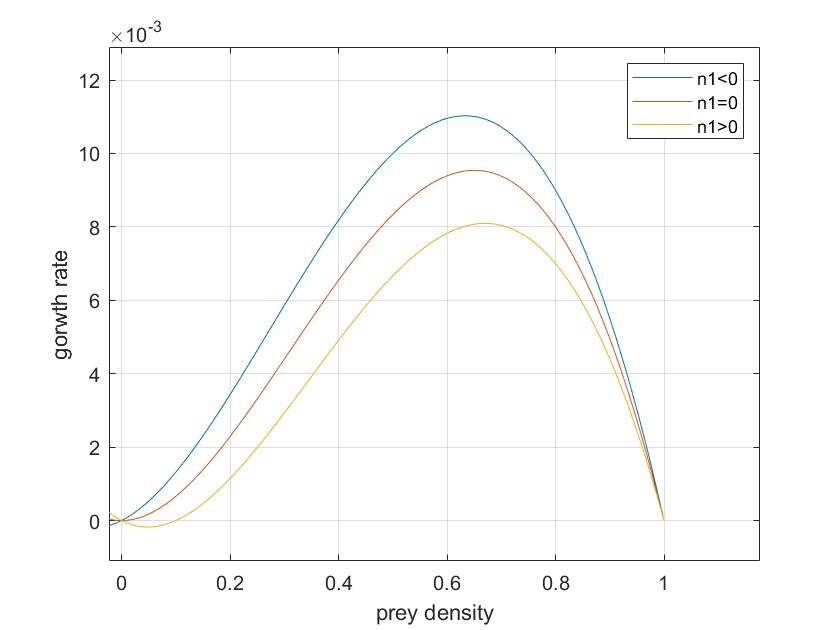
\includegraphics[width=7.5cm]{Allee1.jpg}
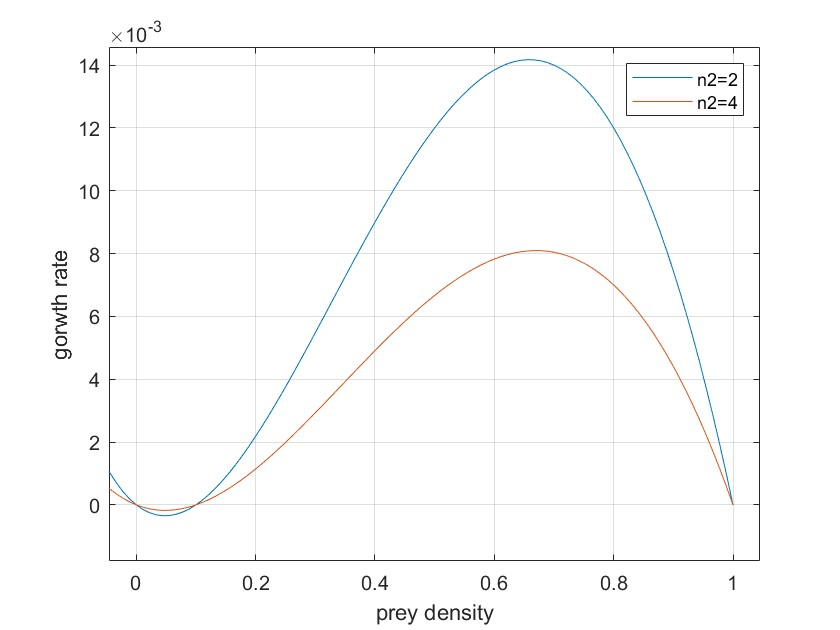
\includegraphics[width=7.5cm]{Allee2.jpg}
\caption{\scriptsize{The growth function of the prey in the absence of predator. (a) The effect of n (n = 2 and 4) in the demographic Allee effect. (b) The weak Allee effect (m $<$ 0 and m = 0) and strong Allee effect (m $>$
 0).}}
\label{fig:my_label}
\end{figure}
\vspace{12pt}
\noindent The left picture above show that: the growth rate of prey can increase fast to a peak value and then goes down, and the rates of prey have the fastest growth while $n_1$ is less than 0, the slowest growth while $n_1$ is greater than 0, and a steady growth rate between these while $n_1$ equals to 0. The right picture shows the situation when $n_2$ belongs to the interval [2,4] (to simplify the model we take the extreme value of this interval), picture demonstrates that the speed of growth rate of prey density increases faster while $n_2$ is small and slower while $n_2$ is larger.These two pictures both show the relationships between growth rate and prey density under different Allee Effect constant ($n_1, n_2$), which is useful to expand the following work.
\vspace{24pt}

\subsubsection{Analyses of Partial Differential Equations Meaning}


$$\frac{dx}{dt}=rx(1-\frac{x}{k})(1-\frac{n_1+n_2}{x+n_2})$$

\vspace{12pt}
\noindent The constant $n_i$ is used in this expression, while the $n_i$ increasing, it becomes stronger to strong Allee effect. $\frac{dx}{dt}$ means the change of trend of the density of population, so it should equal to growth minus death, 
\vspace{12pt}
$$\frac{mxy}{ax+c}$$ 

\vspace{12pt}
\noindent which means the decrease of prey population influenced by the predators. In this expression. there are two assumptions: the number and density of predator always stay in the saturation equilibrium as long as the existence of prey, and the prey can not die naturally, only can be predated.
\vspace{12pt}\\
$\frac{dy}{dt}$ has the same meaning as the $\frac{dx}{dt}$, which can be generated by the following equation:\\

$$\frac{dy}{dt}=\frac{emxy}{ax+c}-dy-hy^2$$\\

\noindent the first term of the right equation is conversion rate times predatory density. Second is death natural density and the third is decreasing with strong competition of the predator. According to the principle of nature, the predator must have more energy to maintain its life and there exists a conversion rate e.

\vspace{24pt}

\subsection{Reaction-diffusion Predator-prey Model with Allee Effect}

\noindent In this part, Partial differential equations are added to a reaction-diffusion term, which can let original PDEs oscillate near the equilibrium points generated by the original PDEs. we can study more precisely with the reaction-diffusion term and simulate the real world. In the current project, the spatiotemporal behaviors of the prey-predator system are described under a uniform environment, i.e. the system parameters do not depend on space or time. To consider this we study the following system of partial differential equations: 
\vspace{12pt}
$$\frac{dx}{dt}=rx(1-\frac{x}{k})(1-\frac{n_1+n_2}{x+n_2})-\frac{mxy}{ax+c}+D_x\nabla^2x$$\\
$$\frac{dy}{dt}=\frac{emxy}{ax+c}-dy-hy^2+D_y\nabla^2y$$\\

\noindent where $D_x$ and $D_y$ are the diffusion coefficient of prey and predator respectively. We assume that $(\overline{n}.\nabla)(x,y)^T=0$, on $\partial\overline\Omega$, where $\partial\overline\Omega$ is the closed boundary of the reaction diffusion domain $\overline\Omega$ and $\overline{n}$ is the outwards unit normal vector to $\partial\overline\Omega$. We assume zero flux boundary conditions which imply a closed system, no species enter or leave the defined environment.
\vspace{12pt}

\noindent To conclude this portfolio of PDEs, obviously, it is related to the density of the population of prey and predator, so the final goal of this study is to find the population density relationship, and Turing conditions, and generate the pictures via MATLAB with an analytical method and numerical method.

\vspace{24pt}

\subsection{Turing Pattern}
\subsubsection{Introduction to Turing Pattern}
\noindent When Turing \footnote{Alan Mathison Turing: British mathematician and logician, known as the father of computer science and artificial intelligence.} was 39 in 1951, he turned to mathematical biology and published his famous masterpiece, "The Chemical Basis of Morphogenesis". It described how patterns in nature, such as stripes and spirals, naturally arise from a uniform state. This story, known as the"morphogenetic reaction-diffusion theory", has become the basic model of theoretical biology, and this pattern is called the "Turing Pattern".

\vspace{24pt}

\noindent The Turing model is interested in the development of forms, patterns, and shapes, as well as their biological organisms. Turing believes that a system in which chemical substances react with each other and diffuse in space is called a reaction-diffusion system, which can explain "the main phenomenon of morphogenesis".
\vspace{12pt}
\begin{figure}[H]
\centering
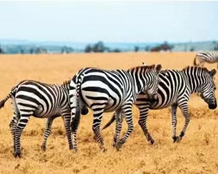
\includegraphics[width=7cm]{zebra.png}
\caption{The manifestation of Turing patches on zebras in nature}
\label{fig:my_label}
\end{figure}


\noindent He used partial differential equations to simulate catalytic reactions in chemistry. For example, if a chemical reaction requires catalyst A, and if the reaction produces more catalyst A, the reaction is auto-catalytic, and there is positive feedback that can be modeled using nonlinear differential equations.

\begin{figure}[H]
\centering
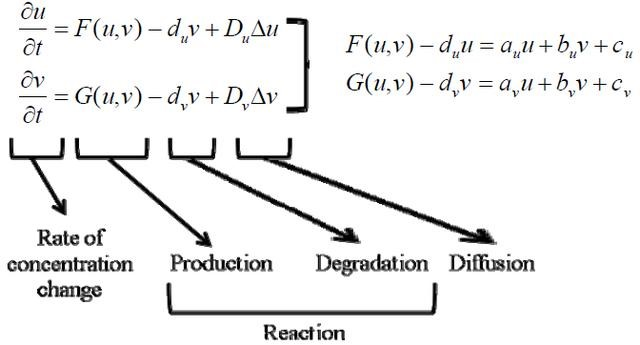
\includegraphics[width=9cm]{Formula in 2.3.1.jpg}
\caption{Examples of catalysts in PDEs}
\label{fig:my_label}
\end{figure}
\vspace{12pt}

\noindent Turing found that patterns maybe produced if the chemical reaction produces catalyst A and inhibitor B, which slows down the production of A. If A and B diffuse through the container at different rates, areas where A and B dominate may be the region where patterns will be generated.
\vspace{24pt}

\noindent To calculate this degree, Turing originally needed a powerful computer, but in 1951 it was not so easy, so he had to manually solve the equations using linear approximation methods. These calculations give correct qualitative results and produce, for example, strange uniform mixed uniform regular fixed spots. The specific working principle diagram is shown in the following figure\footnote{The picture is taken from websites.}.

\begin{figure}[H]
\centering
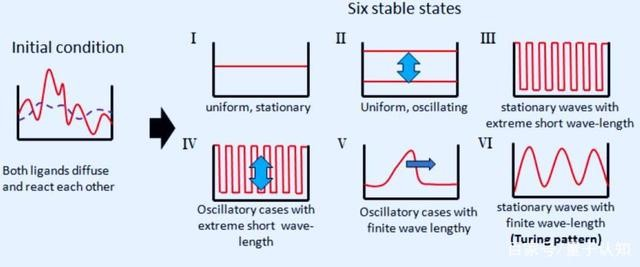
\includegraphics[width=10cm]{wave box.jpg}
\caption{The basic principles of Turing's calculations}

\end{figure}
\vspace{24pt}
\subsubsection{Analytic Method}
\noindent In this project, the spatiotemporal behaviors of the prey-predator system are described under a uniform environment, i.e. the system parameters do not depend on space or time. We want to determine whether this system would have Turing patterns or not.
\vspace{12pt}
\noindent Consider the following system of partial differential equations (PDEs)
$$\frac{dx}{dt}=rx(1-\frac{x}{k})(1-\frac{n_1+n_2}{x+n_2})-\frac{mxy}{ax+c}+D_x\nabla^2x$$\\
$$\frac{dy}{dt}=\frac{emxy}{ax+c}-dy-hy^2+D_y\nabla^2y$$\\


\vspace{24pt}\\

\noindent where $D_x$ and $D_y$ are the diffusion coefficient of prey and predator respectively.\\

\noindent We assume that $(\overline{n}.\nabla)(x,y)^T=0$, on $\partial\overline\Omega$, where $\partial\overline\Omega$ is the closed boundary of the reaction diffusion domain $\overline\Omega$ and $\overline{n}$ is the outwards unit normal vector to $\partial\overline\Omega$. We assume zero flux boundary conditions which imply a closed system, no species enter or leave the defined environment.
\vspace{24pt}

\noindent To determine whether there exist Turing patterns in the given system, we try to compute the Turing instability\footnote{Turing instability: a quantity to decide whether a differential-equations system has Turing patterns or not.} below. We will consider the problem with the Neumann Boundary Condition\footnote{Neumann Boundary Condition: a very famous boundary condition to solve differential problem, we will not discuss it in this paper but the condition-equation was given.} .

$$x_x(0,t) = x_x(L,t) = y_x(0,t) = y_x(L,t)$$
\vspace{12pt}

\noindent First, we rewrite the system for convenience:

$$\textbf{u}= (x,y)^T\\$$

$$
\textbf{F(u)} = (f,g)^T = 
\begin{pmatrix}
rx(1-\frac{x}{k})(1-\frac{n_1+n_2}{x+n_2})-\frac{mxy}{ax+c}\\

\frac{emxy}{ax+c}-dy-hy^2
\end{pmatrix}
$$
\vspace{12pt}
$$
\textbf{D} = \begin{pmatrix}
D_x&0\\
0&D_y
\end{pmatrix}
$$
\vspace{12pt}

\noindent which satisfies that

$$
\textbf{U}_t = \textbf{F(u)} + \textbf{D}\nabla^2\textbf{u}
$$
\vspace{12pt}

\noindent Let $u^*$ be the solution of $\textbf{F}(\textbf{u}) = 0$. Then $u^*$ is a spatially homogeneous equilibrium solution of the ODE model(when \textbf{D} = 0)

$$\textbf{u}^* = (x^*,y^*)$$
$$\frac{d\textbf{u}}{dt} = \textbf{F}(\textbf{u)}$$
$$\frac{d\textbf{u}}{dt}|_{u=u^*} = \textbf{F}(\textbf{u}^*) = 0
$$
\vspace{12pt}

\noindent For Turing instability, we require that $u^*$ be a locally stable solution of the ODE model but an unstable solution of the PDE model. To find conditions for this situation occurs, we let $\textbf{w} = \textbf{u} - \textbf{u}^*$. Notice that, 

\begin{align*}
  \frac{d\textbf{w}}{dt} &= \frac{d(\textbf{u} - \textbf{u}^*)}{dt}\\
    &= \frac{d\textbf{u}}{dt} - \frac{d\textbf{u}^*}{dt} \\
    &= \textbf{F}(\textbf{u}) - \textbf{F}(\textbf{u}^*) \\
    &= \textbf{F}(\textbf{u}^*) + \textbf{Jw}
\end{align*}


\noindent After linearizing we obtain,
\vspace{12pt}

$$
\textbf{w}_t = \textbf{F}(\textbf{u}^*) + \textbf{Jw} + \textbf{Dw}_{xx}
$$
\vspace{12pt}

\noindent where J is the Jacobian Matrix of the system evaluated at $u^*$, given by
\vspace{12pt}

$$
\textbf{J}=
\begin{pmatrix}
f_x&g_y\\
g_x&g_y
\end{pmatrix}
|_{\textbf{u}=\textbf{u}^*}
$$
\vspace{12pt}

\noindent Since $\textbf{F}(\textbf{u}^*) = 0$, the linearized system becomes
\vspace{12pt}

$$
\textbf{w}_t=\textbf{Jw}+\textbf{D}\textbf{w}_{xx}.
$$
\vspace{12pt}

\noindent We can search for a solution in the form of a sum of separable solutions. We consider a general separable solution,  
\vspace{12pt}

$$
w(x,t)=T(t)X(x)\textbf{c}
$$
\noindent with a constant vector c.
\vspace{12pt}


\noindent Here we assume that T(x) and X(x)are scalar functions of t and x respectively and c is a $2\times1$ constant vector. Substituting in the system and dividing by T(t)X(x), we obtain
\vspace{12pt}

$$
\dfrac{\dot T}{T}c=D\dfrac{\ddot X}{X}c+\text{J}c.
$$
\vspace{12pt}

\noindent For this equation to hold, $\dfrac{\dot T}{T}$  must be a quantity independent of t. Hence it must be a constant, say $\lambda$. Similarly, $\dfrac{\ddot X}{X}$ must be another constant, say $-k^2$. So we have that
\vspace{12pt}

$$
T(t)=T_0e^{\lambda t}
$$
\vspace{12pt}

\noindent We also have that
\vspace{12pt}

$$
\begin{array}{ll}&X''+k^2X=0\\  
\\&X'''(0)=X''(L)=0.\end{array}
$$
\vspace{12pt}

\noindent There is only one independent variable of function X, it is a very common ODE problem to solve. Here, the result is given. In particular,
\vspace{12pt}

$$
\begin{matrix}k_n=\dfrac{n\pi}{L},\\  \\
X_n(x)=A_n\cos(k_nx).\end{matrix}
$$
\vspace{12pt}

\noindent Next, we put the solution mentioned before back to the equations, we can get the following equations:
\vspace{12pt}

$$
\lambda c = -Dk^2c + \text{J}c,
$$
\vspace{12pt}

\noindent which will have a solution if and only if 
\vspace{12pt}
$$
|\mathrm{J}-Dk^2-\lambda I|=0,
$$
\vspace{12pt}

\noindent where I is the $2\times2$ identity matrix. In expanded form, this determinant is,
\vspace{12pt}

$$
\begin{vmatrix}f_x-D_xk^2-\lambda&f_y\\ g_x&g_y-D_yk^2-\lambda\end{vmatrix}=0
$$
\vspace{12pt}

\noindent This gives the following quadratic equation in $\lambda$:
\vspace{12pt}

$$
\lambda^2+\left[\left(D_{x}+D_{y}\right)k^2-\left(f_{x}+g_{y}\right)\right]\lambda+\left[D_{x}D_{y}k^4-\left(D_{y}f_{x}+D_{x}g_y\right)k^2+\left(f_{x}g_{y}-f_{y}g_{x}\right)\right]=0\quad
$$
\vspace{12pt}

\noindent When the diffusion coefficients are not zero, the conditions for stability of the determinant for each $k_n$ are
\vspace{12pt}

$$
\begin{array}{l}f_x+g_y-\big(D_x+D_y\big)k^2<0,\\ \\ (f_x-D_x k^2)\big(g_y-D_y k^2\big)-f_y g_x>0.\end{array}
$$
\vspace{12pt}

\noindent Because of assumptions, the first inequality above is always satisfied. Thus, the only way we may destabilize the diffusion equilibrium with the diffusion is if we find that
\vspace{12pt}

$$
(f_x-D_x k^2)\big(g_y-D_yk^2\big)-f_yg_x<0
$$
\vspace{12pt}

\noindent The left-hand side of that inequality is a quadratic function of $k^2$:
\vspace{12pt}

$$
H(k^2)=Ak^4-Bk^2+C,
$$
\vspace{12pt}

\noindent where $A=D_x D_y$, B = $D_y f_x+g_y D_x$, C = $f_x g_y-f_y g_x$.
\vspace{12pt}

\noindent We conclude that stability occurs if the roots of the quadratic function are real.
\vspace{12pt}

\noindent Let

$$
\mu=k^2,where \mu\in[0,\infty],
$$
\vspace{12pt}

\noindent then we rewrite the function

$$
h(\mu)=A\mu^{2}-B\mu+C.
$$
\vspace{12pt}

\noindent We say the roots are $\mu_1, \mu_2$ respectively, there exists a solution such that $\mu \in [\mu_1,\mu_2]$. Therefore, Turing instability occurs if

$$
B>0 $$
and

$$
B^2>4AC.
$$
\vspace{12pt}

\noindent The first inequality holds to satisfy the axis of symmetry of the function will be in positive axis, since $\mu\in\left[0,\infty\right]$, there cannot be two negative roots. The second inequality holds to satisfy there are two real roots.
\vspace{12pt}\\
Therefore, we want 
\vspace{12pt}

$$
\begin{array}{c}D_y f_x+g_y D_x>0\\ \\ D_y f_x +g_y D_x>2\sqrt{D_x D_y(f_x g_y-f_y g_x)}\\ \end{array}
$$
\vspace{12pt}

\noindent Notice that the first condition cannot hold if $D_y = D_x$. That is why for Turing instability we always need very distinct diffusion rates. 
\vspace{24pt}\\
If both of the two inequalities above hold at the same time, there will occur two situations\footnote{ Two situations: the pictures of both two situations are just examples which are generated by randomly
exact values.} we need to consider.
\vspace{24pt}\\
The first situation is that the two roots are both positive, then we can take the range [$\mu_1,\mu_2$] for the Turing instability.
\vspace{12pt}\\


\begin{figure}[H]
\centering
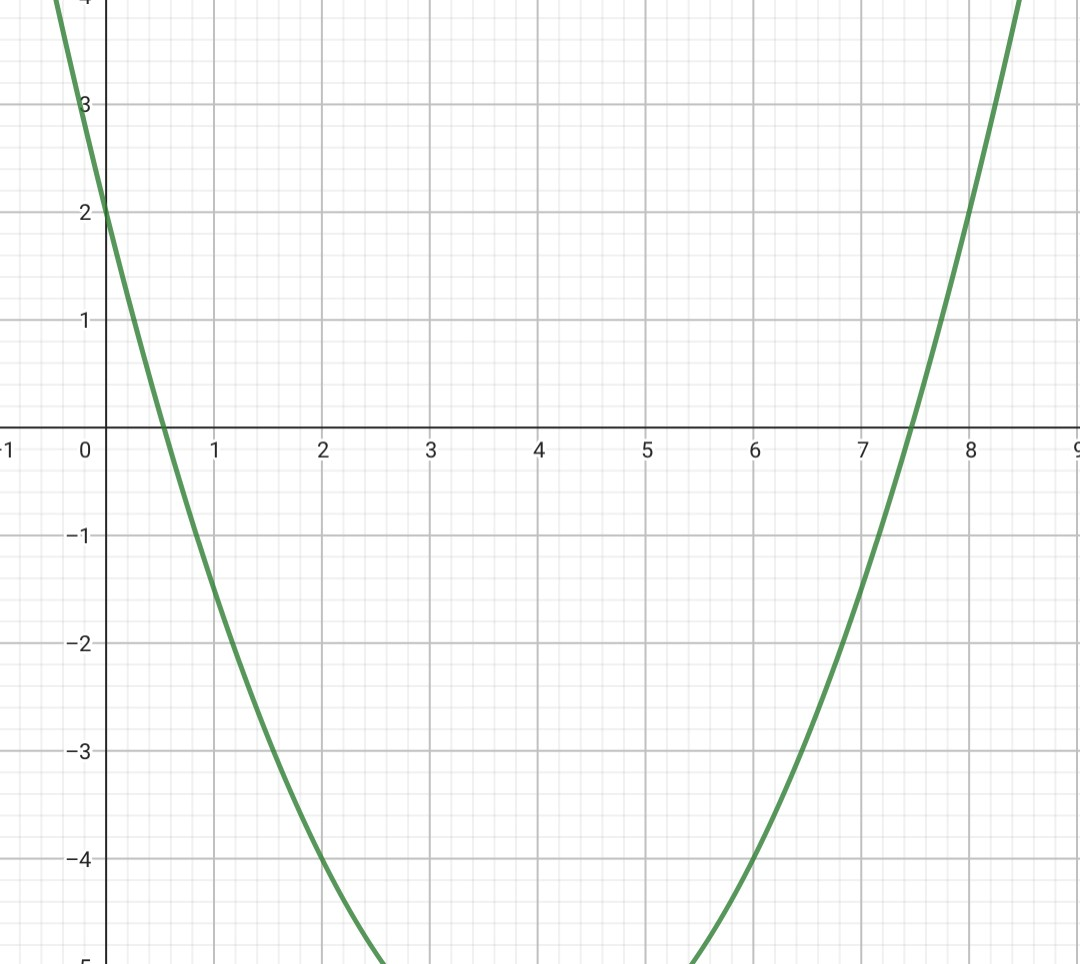
\includegraphics[width=7cm]{1.jpg}
\caption{The first situation}
\label{fig:my_label}
\end{figure}


\noindent The second situation is that there is one positive root but another root is negative. Since $\mu \in [0, \infty]$, we cannot take the range as $\left[\mu_1,\mu_2\right]$ like before, we need to change our range into $[0,\mu_2]$.
\vspace{12pt}

\begin{figure}[H]
\centering
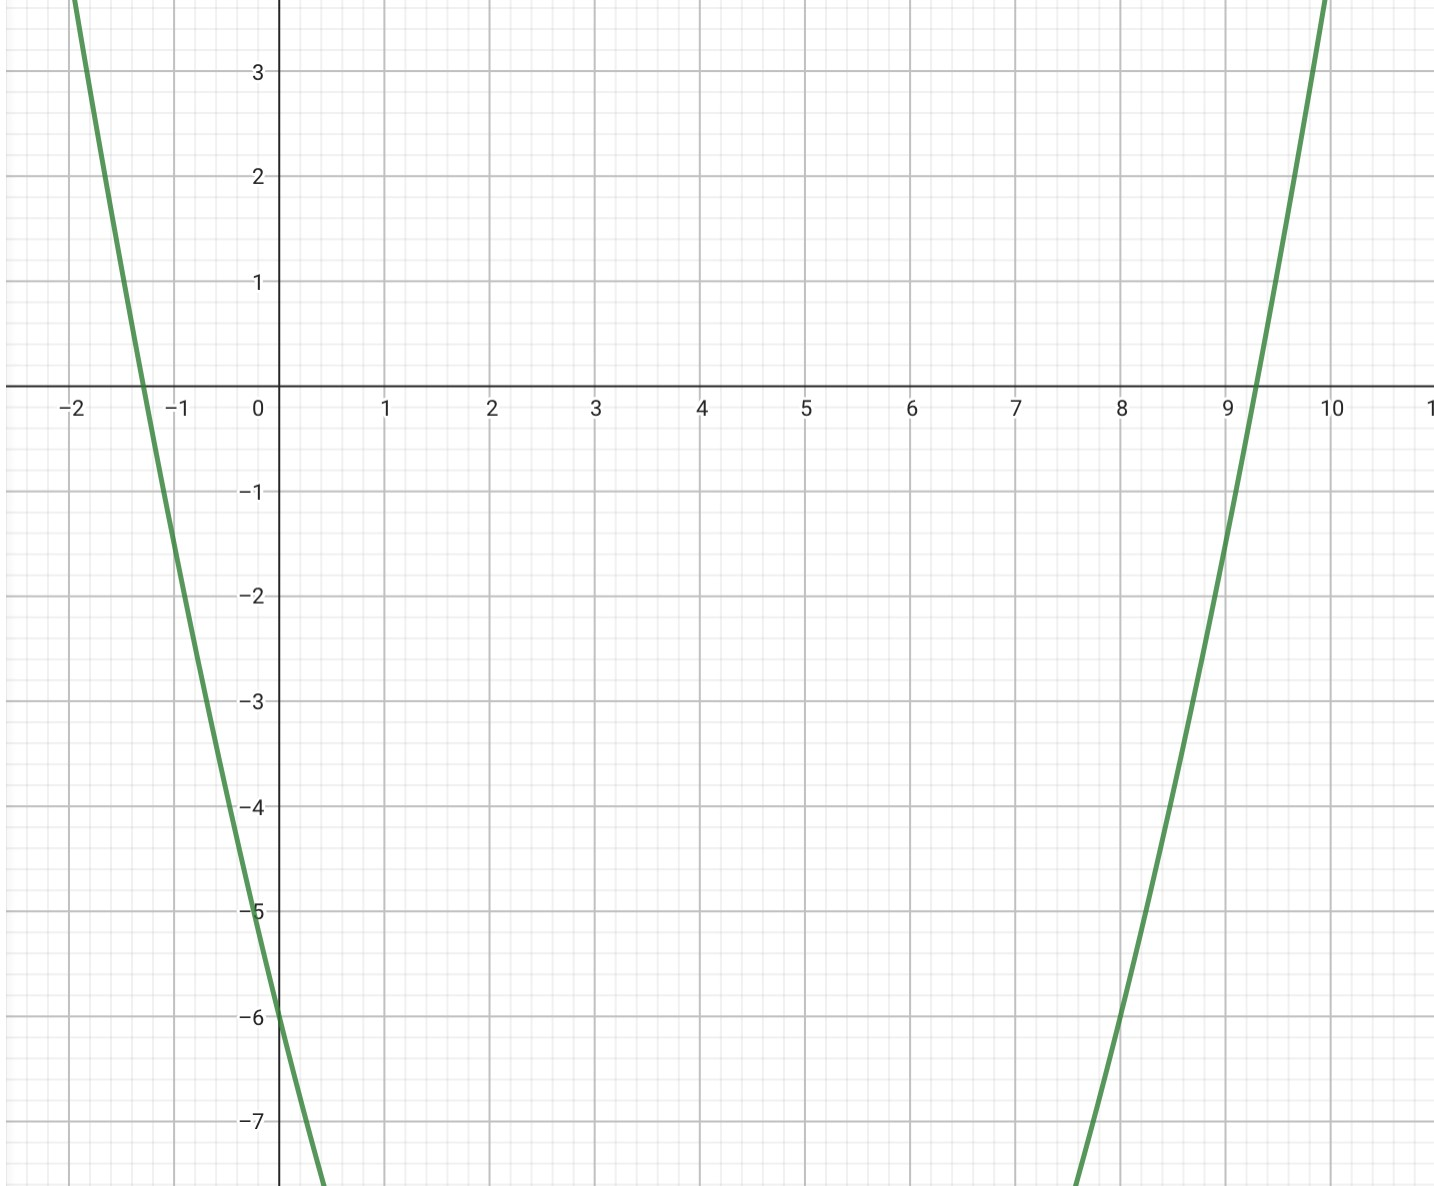
\includegraphics[width=7cm]{2.jpg}
\caption{The second situation}
\label{fig:my_label}
\end{figure}

\noindent We can use François Viète’s theorem\footnote{François Viète’s theorem: illustrate the relationship between roots and coefficients in a quadratic equation of one variable
} to differentiate the two situations. The first situation occurs if and only if
\vspace{12pt}

$$
\mu_{1}\times\mu_{2}>0,
$$
\vspace{12pt}

\noindent which implies that

$$
\dfrac{C}{A}>0.
$$
\vspace{12pt}

\noindent Similarly, the second situation occurs if and only if

$$\dfrac{C}{A}<0.
$$
\vspace{12pt}

\noindent In summary, Turing instability occurs in two different ranges.\\
Firstly, we take the range in [$\mu_1,\mu_2$] if
\vspace{12pt}

$$
\begin{array}{c}D_y f_x+g_y D_x>0\\ \\ D_y f_x +g_y D_x>2\sqrt{D_x D_y(f_x g_y-f_y g_x)}\\ \\ \frac{f_x g_y -f_y g_x}{D_x D_y}>0.\end{array}
$$
\vspace{12pt}

\noindent Secondly, we take the range in [$0,\mu_2$] if

$$
\begin{array}{c}D_y f_x+g_y D_x>0\\ \\ D_y f_x +g_y D_x>2\sqrt{D_x D_y(f_x g_y-f_y g_x)}\\ \\ \frac{f_x g_y -f_y g_x}{D_x D_y}<0.\end{array}
$$
\vspace{12pt}

\noindent Notice that, since $\mu = k^2$, where $\mu\in[0,\infty]$, after we find the value of ${k_1}^2\&{k_2}^2$, we need to determine the exact value of $k_1$ and $k_2$.
\vspace{12pt}

\noindent Remark that
$$
F(\boldsymbol{u})=(f,g)^T=\begin{pmatrix}rx\left(1-\frac{x}{k}\right)\left(1-\frac{n_1+n_2}{x+n_2}\right)-\frac{mxy}{ax+c}\\ \frac{emxy}{ax+c}-dy-hy^2\end{pmatrix},\quad
$$
so
$$
f_x=r\left(1-\dfrac{2x}{k}\right)\left(1-\dfrac{{n_1+n_2}}{{x+n_2}}\right)+rx\left({1-\dfrac{x}{k}}\right)\left({1+\dfrac{n_1+n_2}{(x+n_2)^2}}\right)-\dfrac{my(ax+c)-amxy}{(ax+c)^2}\quad
$$
\vspace{12pt}
$$
\begin{aligned}f_y&=-\frac{mx}{ax+c}\\ g_x&=\frac{emy(ax+c)-aemxy}{(ax+c)^2}\\ g_y&=\frac{emx}{ax+c}-d-2hy\end{aligned}
$$
\vspace{12pt}\\
\noindent and $D_x, D_y$ are the diffusion of two variables respectively. Therefore, to satisfy the inequality, we let
\vspace{12pt}

\begin{equation}
\begin{aligned}
E_1 =& D_y \left[ r(1-\frac{2x}{k})(1-\frac{n_1+n_2}{x+n_2})+rx(1-\frac{x}{k})(1+\frac{n_1+n_2}{(x+n_2)^2})-\frac{my(ax+c)-amxy}{(ax+c)^2}\right] \\
&+D_X\left[ \frac{emx}{ax+c}-d-2hy\right]\\
\end{aligned}
\end{equaiton}


\begin{equation*}
\begin{aligned}
E_2 =&  \left[ r(1-\frac{2x}{k})(1-\frac{n_1+n_2}{x+n_2})+rx(1-\frac{x}{k})(1+\frac{n_1+n_2}{(x+n_2)^2})-\frac{my(ax+c)-amxy}{(ax+c)^2}\right]\\ &\left[ \frac{emx}{ax+c}-d-2hy\right]-\left[-\frac{mx}{ax+c}\right] \left[\frac{emy(ax+c)-aemxy}{(ax+c)^2}\right],\\ \\
\end{aligned}
\end{equaiton*}

\vspace{12pt}

\noindent and we let
\vspace{12pt}

\begin{equation*}
\begin{aligned}&I_1=E_1\\ &I_2=E_1-2\sqrt{D_xD_yE_2}\\ &I_3=\frac{E_2}{D_xD_y}.\\ \\
\end{aligned}
\end{equation*}

\noindent Now, if we want Turing instability to occur in the two different situations,


\noindent if the first situation occurs, then
\vspace{12pt}

\begin{equation*}
\begin{aligned*}
\begin{cases}I_1>0\\I_2>0\\I_3>0,\end{cases}\\
\end{aligned*}
\end{equation*}

\vspace{12pt}

\noindent if the second situation occurs, then
\begin{equation*}
\begin{aligned*}
\begin{cases}I_1>0\\I_2>0\\I_3<0.\\ \end{cases}
\end{aligned*}
\end{equation*}

\vspace{24pt}

\subsubsection{Computation based on data}
\noindent After determining the mathematical equations, we need the measurements of each parameter to find out the exact value of the function, also the characteristics of each functions can be seen.\\
\vspace{24pt}

\noindent The mentioned parameters\footnote{Metioned parameters: the parameters which were mentioned in the introduction, e.g. prey intrinsic growth rate $\textit{r}$, etc.} are randomly determined within a desirable template in corresponding papers. In the report, we referred to our mentor Mainul Haque's\footnote{Mainul Haque: World’s Top 2$\%$ Scientist} suggestions, we take (without unit):
\vspace{12pt}

\begin{table}[htbp]
    \centering
    \begin{tabular}{|c|c|}
    \hline
r&0.8\\
\hline
k&100\\
\hline
m&24\\
\hline
e&0.33\\
\hline
d&0.1\\
\hline
a&15\\
\hline
c&30\\
\hline
h&0.01\\
\hline
$n_2$&10\\
\hline
\end{tabular}
\caption{Value Selection of Constants}
\label{tab:my_label}
\end{table}
\vspace{24pt}

\subsection{Numerical Analysis}
\noindent For the vector-valued function
\vspace{12pt}

$$
\textbf{F(u)} = (f,g)^T = 
\begin{pmatrix}
rx(1-\frac{x}{k})(1-\frac{n_1+n_2}{x+n_2})-\frac{mxy}{ax+c}\\
\\
\frac{emxy}{ax+c}-dy-hy^2
\end{pmatrix}
$$
\vspace{12pt}

\noindent we want to seek an equilibrium point based on the table above, so we need to
find
\vspace{12pt}

\begin{equation*}
\frac{\partial x}{\partial t}=0
\end{equation*}
\begin{equation*}
\frac{\partial y}{\partial t}=0
\end{equation*}
\vspace{12pt}

\noindent when (\textit{x}, \textit{y}) = (\textit{x*, y*}).\\
\vspace{24pt}

\noindent With different inputs of $n_1$, we compute the equilibrium with Matlab, also we use Matlab to compute the value of $I_i$  to satisfy the existence of roots.\\
\vspace{24pt}

\noindent After finding the equilibrium points, we use Matlab to generate the Turing patterns, there are several parameters in the coding, please checked the appendix to find more detailed information. The ‘initial data function’ used in this paper was taken from Marcus R. Garvie’s paper: Finite-Difference Schemes for Reaction–Diffusion Equations Modeling Predator–Prey Interactions in MATLAB.\\ 
\vspace{24pt}

\noindent The value of several parameters had been determined, the only parameter which will be changed is $n_1$. Please notice that, to discuss the Allee Effect, the Allee constant $n_1$ and $n_2$ were always written to be one constant N in many research\footnote{There are many papers to discuss the Allee Effect but with different forms, we do not discuss in detail here}, the form had also been different to this paper. The value of $n_1$ was taken as 10, which is a large number so that the value of $n_2$ should be much smaller than $n_1$ to satisfy the sum of them will be determined as an advisable range. \\
\vspace{24pt}

\noindent With the changing of the value of $n_1$, the spatial impact with time changes of preys and predators caused by the Allee Effect will be shown. Before that, the value of $n_1$ should be checked by the constructed \textit{ineqn} mentioned before.\\




\begin{table}[h]
\centering
\begin{tabular}{|c|c|c|c|}
\hline
\textbf{\begin{tabular}[c]{@{}c@{}}The value of\\  $n_1$\end{tabular}}                   & \textbf{0.1}    & \textbf{0.2}    & \textbf{0.3}    \\ \hline
\multirow{7}{*}{\textbf{\begin{tabular}[c]{@{}c@{}}The value of $(x,y)$\end{tabular}}} & (0,0)           & (0,0)           & (0,0)           \\ \cline{2-4} 
& (-2,0)          & (-2,0)          & (-2,0)          \\ \cline{2-4} 
& (0.-10)         & (0.-10)         & (0.-10)         \\ \cline{2-4} 
& (100,0)         & (100,0)         & (100,0)         \\ \cline{2-4} 
& (0.1,0)         & (0.2,0)         & (0.3,0)         \\ \cline{2-4} 
& (-9.337,57.198) & (-9.332,57.202) & (-9.326,57.214) \\ \cline{2-4} 
& (0.469,0.043)   & (0.469,0.031)   & (0.468,0.019)   \\ \hline
\end{tabular}
\caption{Test Result 1}
\end{table}

\noindent There were several imaginary roots which had been ignored.\\
\vspace{24pt}

\noindent It would be meaningless to draw the diagrams based on some ‘extreme roots’ given above, for example, the value of (\textit{x,y}) is \textbf{0} if and only if there was no prey or predator initially. In fact, any of the value of x or y can not be 0. Also, the roots with negative value were also meaningless in biologism, since there could not be negative numbers of living beings. In summary, the values which should be considered were only:
\vspace{24pt}

\begin{equation*}
    (0.469, 0.043); (0.469, 0.031); (0.468, 0.019).
\end{equation*}
\vspace{12pt}

\noindent The diffusion coefficients were taken as $D_x=0.03,D_y=3$,
\vspace{12pt}

\begin{table}[h]
\centering
\begin{tabular}{|l|l|l|l|}
\hline
$n_1$=0.1 & $I_1$=1.233 & $I_2$=1.206  & $I_3$=0.022 \\ \hline
$n_1$=0.2 & $I_1$=1.230 & $I_2$=1.2067 & $I_3$=0.016 \\ \hline
$n_1$=0.3 & $I_1$=1.234 & $I_2$=1.206  & $I_3$=0.009 \\ \hline

\end{tabular}
\caption{Test Result 2}
\end{table}
\vspace{12pt}

\noindent Based on the test results, all of these $n_1$ can be used to generate the Turing patterns graphs. The coding was taken from the given reference. The parameters were taken as the same as mentioned table. The area was taken in (0, 400), the space step was 15, the time step was $\frac{1}{24}$, the maximum time was 120, and the parameter delta would be the value of $\frac{D_y}{D_x}$, which was 100.\\

\noindent When $n_1=0.1$ (u is the ‘prey x’, v is the ‘predator y’),

\begin{figure}[H]
\centering
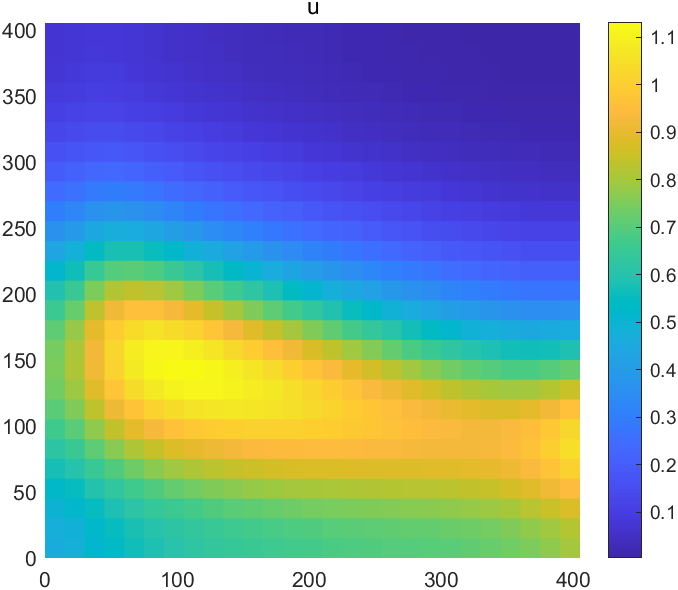
\includegraphics[width=6.8cm]{1.1.png}
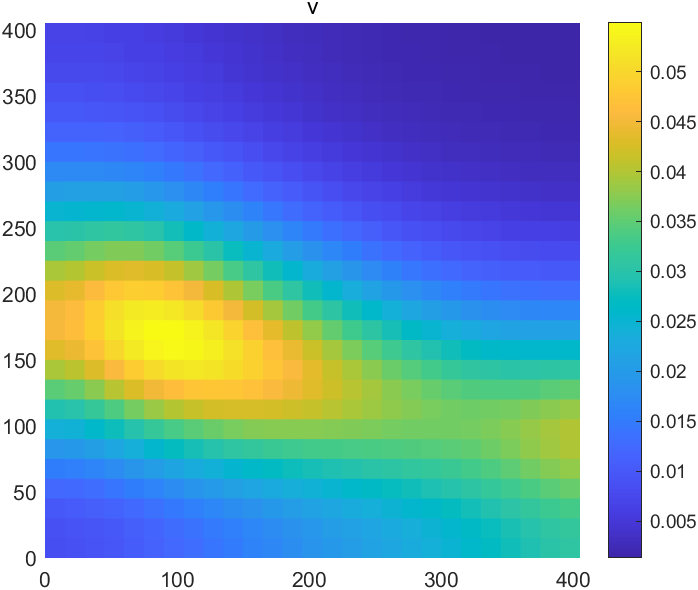
\includegraphics[width=7cm]{1.2.png}
\caption{$n_1 = 0.1$, side length = 400, space step = 15, time step = 1/24, maximum time = 120, Dy/Dx = 100, $u^* = 0.469, v^* = 0.043$, $U_{i,j}^0 = u^*-2\times10^{-7}(x_i-0.1y_j-225)(x_i-0.1y_j-675), V_{i,j}^0 = v^*-3\times10^{-5}(x_i-450)-1.2\times10^{-4}(y_i-150)$}
\end{figure}
\vspace{12pt}

\noindent when $n_1=0.2$,

\begin{figure}[H]
\centering
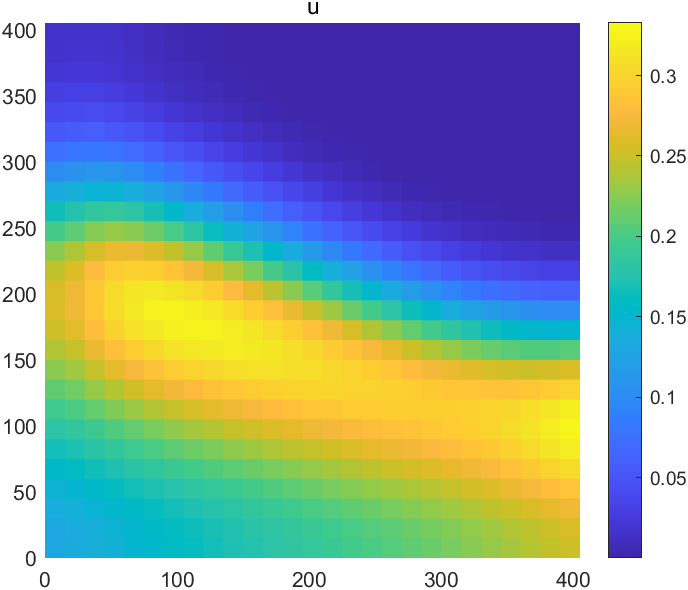
\includegraphics[width=7cm]{2.1.png}
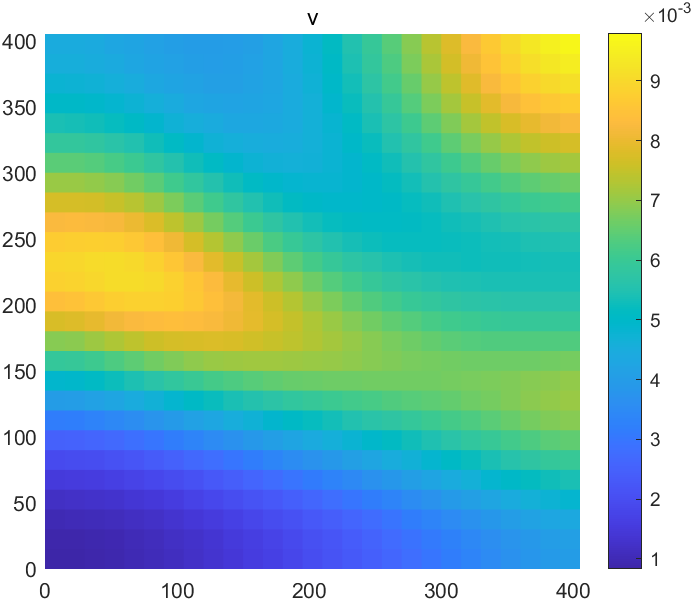
\includegraphics[width=7cm]{2.2.png}
\caption{$n_1 = 0.2$, side length = 400, space step = 15, time step = 1/24, maximum time = 120, Dy/Dx = 100, $u^* = 0.469, v^* = 0.031$, $U_{i,j}^0 = u^*-2\times10^{-7}(x_i-0.1y_j-225)(x_i-0.1y_j-675), V_{i,j}^0 = v^*-3\times10^{-5}(x_i-450)-1.2\times10^{-4}(y_i-150)$}
\end{figure}

\noindent when $n_1=0.3$,
\begin{figure}[H]
\centering
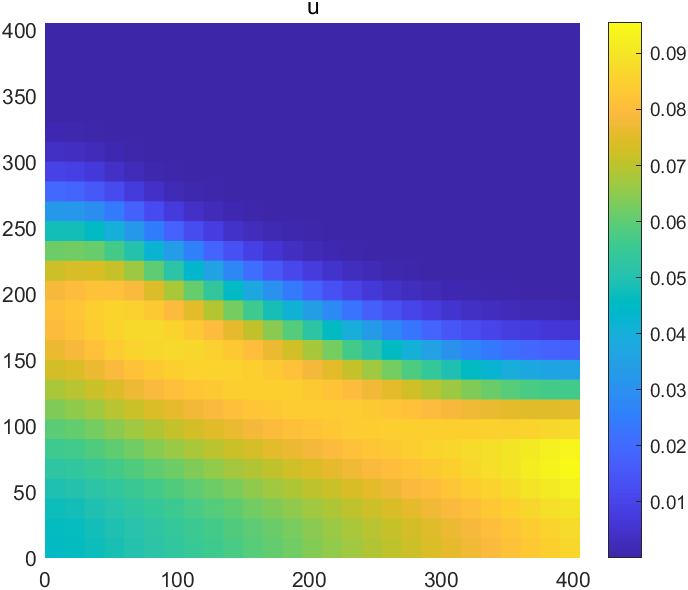
\includegraphics[width=7cm]{3.1.png}
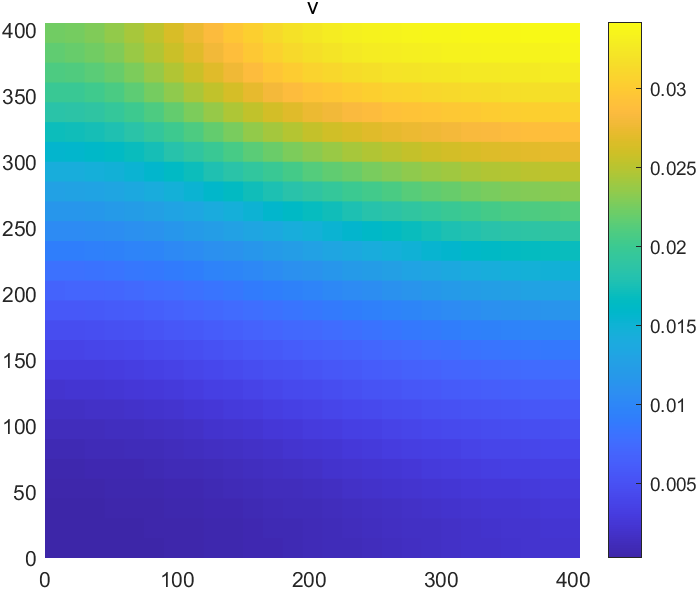
\includegraphics[width=7cm]{3.2.png}
\caption{$n_1 = 0.3$, side length = 400, space step = 15, time step = 1/24, maximum time = 120, Dy/Dx = 100, $u^* = 0.468, v^* = 0.019$, $U_{i,j}^0 = u^*-2\times10^{-7}(x_i-0.1y_j-225)(x_i-0.1y_j-675), V_{i,j}^0 = v^*-3\times10^{-5}(x_i-450)-1.2\times10^{-4}(y_i-150)$}
\end{figure}

\noindent From the graphs, it can be seen that, although the changes in the value of $n_1$ were not large, only 0.1 per time, there was a significant impact on the spatial distribution of predators over a certain period time. After more drawings based on different values of $n_1$, if the value was too large or too small, the situations would be different.\\
\vspace{24pt}

\noindent For example, if we take $n_1=0.001$,
\begin{figure}[H]
\centering
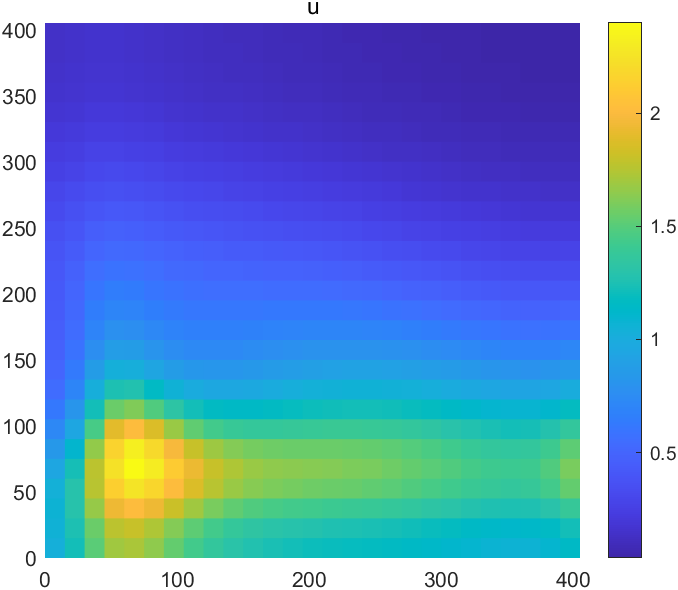
\includegraphics[width=7cm]{4.1.png}
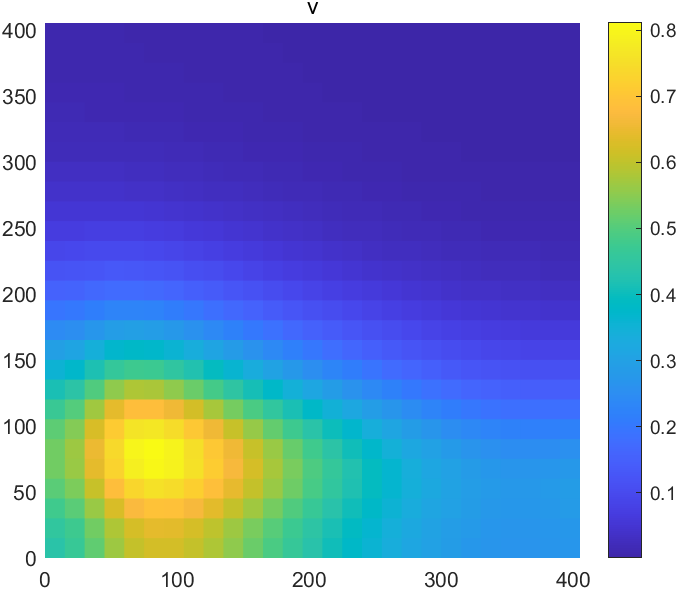
\includegraphics[width=7cm]{4.2.png}
\caption{$n_1 = 0.001$, side length = 400, space step = 15, time step = 1/24, maximum time = 120, Dy/Dx = 100, $u^* = 0.47, v^* = 0.055$, $U_{i,j}^0 = u^*-2\times10^{-7}(x_i-0.1y_j-225)(x_i-0.1y_j-675), V_{i,j}^0 = v^*-3\times10^{-5}(x_i-450)-1.2\times10^{-4}(y_i-150)$}
\end{figure}

\noindent if we take $n_1=0.00001$,
\begin{figure}[H]
\centering
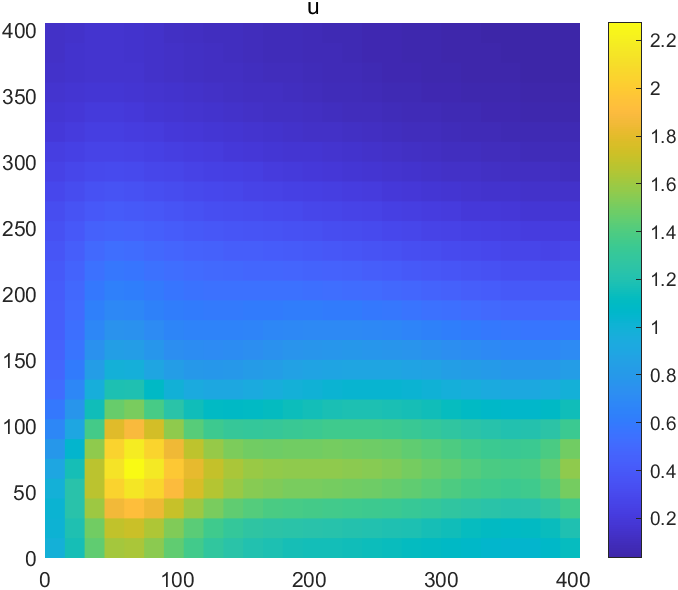
\includegraphics[width=7cm]{5.1.png}
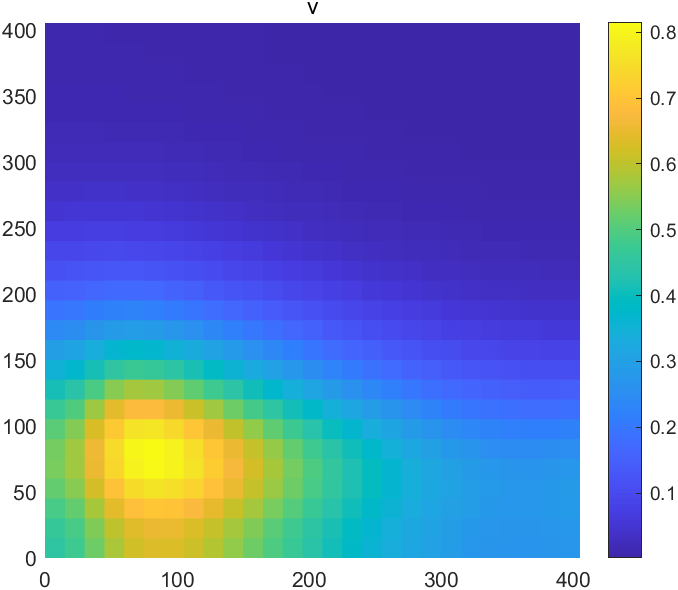
\includegraphics[width=7cm]{5.2.png}
\caption{$n_1 = 0.00001$, side length = 400, space step = 15, time step = 1/24, maximum time = 120, Dy/Dx = 100, $u^* = 0.47, v^* = 0.055$, $U_{i,j}^0 = u^*-2\times10^{-7}(x_i-0.1y_j-225)(x_i-0.1y_j-675), V_{i,j}^0 = v^*-3\times10^{-5}(x_i-450)-1.2\times10^{-4}(y_i-150)$}
\end{figure}

\noindent From this graph, it can be seen that, if we take $n_1$ too small, then the patterns will not change. However, if we take $n_1$ bigger than 0.4, like 0.5 or 0.6, there will be not positive roots to generate the graphs. From now on, we just take the value of $n_2$ in a range.
\vspace{24pt}

\noindent However, if we change the number of $n_2$, the situation will be totally different. We mainly consider in two ways: first, the value of $n_2$ is very big ot tends to infinity; second, the value of $n_2$ is very small or tends to 0.
\vspace{24pt}

\noindent For the first situation, we take $n_2$=1000, under this situation, there also has two choices: taking $n_1$ large or small. Unfortunately, after several times of tests, there will be no appropriate pattern if we take $n_1$ too small, both u and v tends to . Therefore, we take $n_1$ in a large number to generate the patterns:
\vspace{24pt}

\noindent If $n_1$ =1000, there are two sets of roots to generate the patterns,

\begin{figure}[H]
\centering
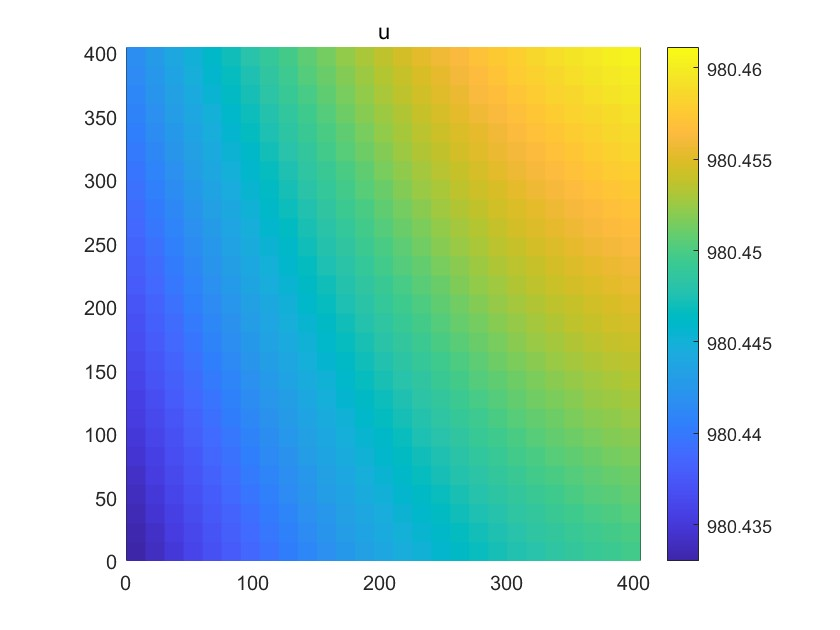
\includegraphics[width=7cm]{out1.jpeg}
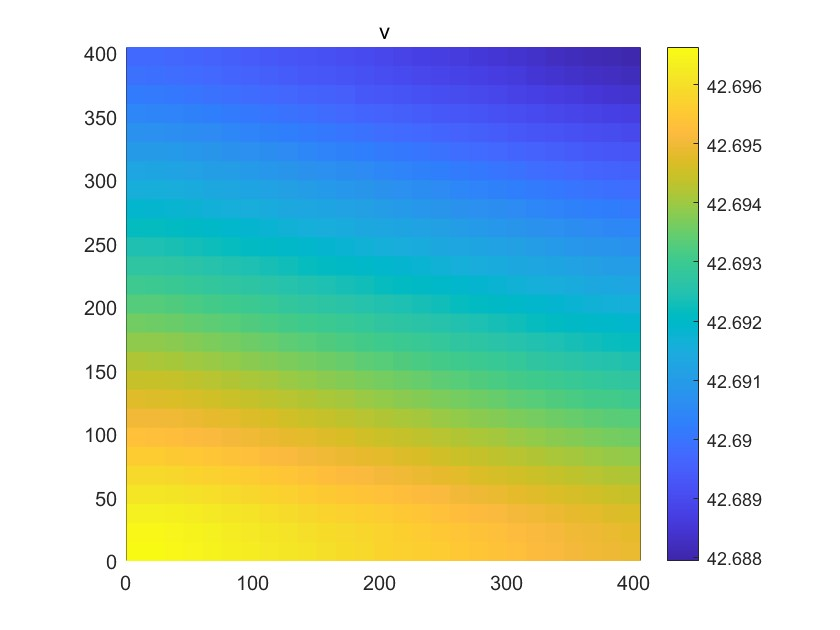
\includegraphics[width=7cm]{out2.jpeg}
\caption{$n_1 = 1000$, side length = 400, space step = 15, time step = 1/24, maximum time = 120, Dy/Dx = 100, $u^* = 169.32, v^* = 42.183$, $U_{i,j}^0 = u^*-2\times10^{-7}(x_i-0.1y_j-225)(x_i-0.1y_j-675), V_{i,j}^0 = v^*-3\times10^{-5}(x_i-450)-1.2\times10^{-4}(y_i-150)$}
\end{figure}

\begin{figure}[H]
\centering
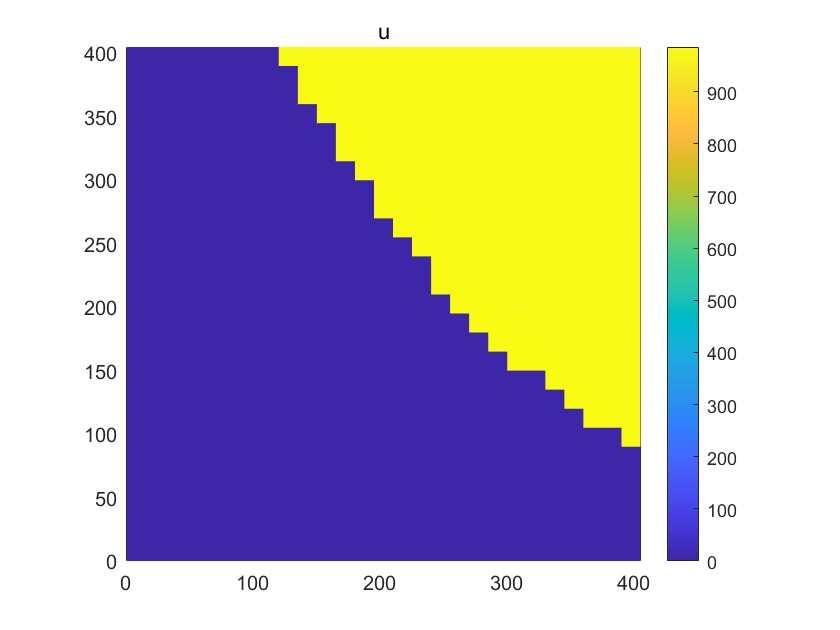
\includegraphics[width=7cm]{out3.jpeg}
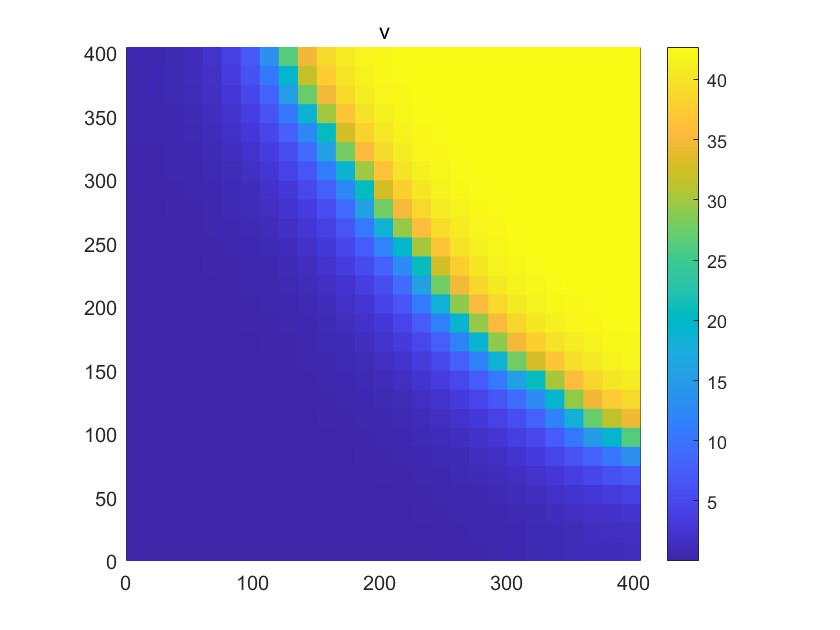
\includegraphics[width=7cm]{out4.jpeg}
\caption{$n_1 = 1000$, side length = 400, space step = 15, time step = 1/24, maximum time = 120, Dy/Dx = 100, $u^* = 980.45, v^* = 42.692$, $U_{i,j}^0 = u^*-2\times10^{-7}(x_i-0.1y_j-225)(x_i-0.1y_j-675), V_{i,j}^0 = v^*-3\times10^{-5}(x_i-450)-1.2\times10^{-4}(y_i-150)$}
\end{figure}

\noindent If $n_1$=10000, there are also two sets of roots,

\begin{figure}[H]
\centering
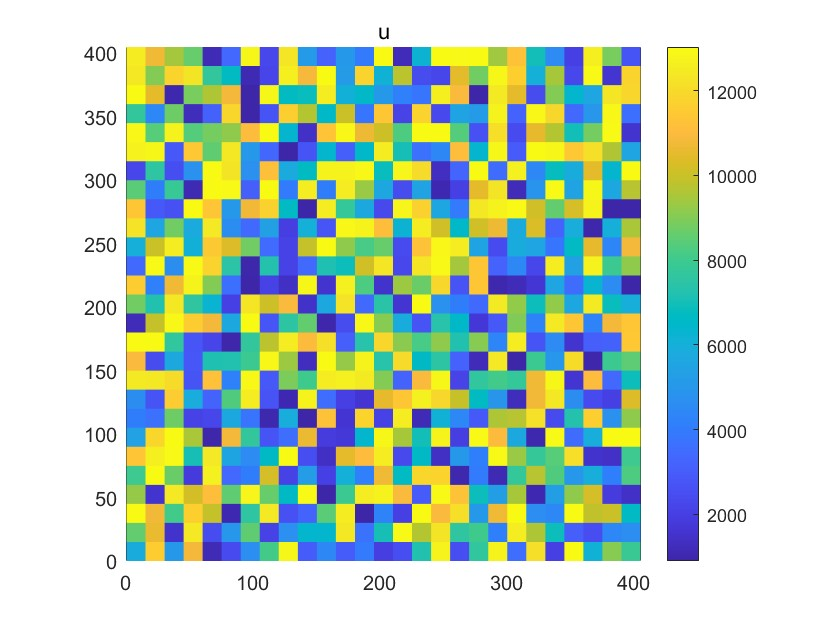
\includegraphics[width=7cm]{out5.jpeg}
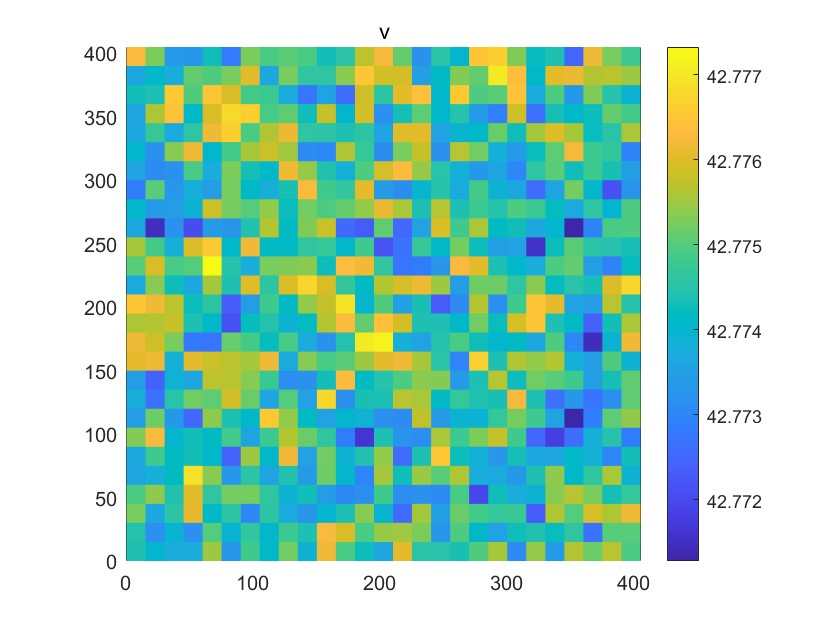
\includegraphics[width=7cm]{out6.jpeg}
\caption{$n_1 = 10000$, side length = 400, space step = 15, time step = 1/24, maximum time = 500, Dy/Dx = 100, $u^* = 9999.04, v^* = 42.789$, $U_{i,j}^0 = u^*-2\times10^{-7}(x_i-0.1y_j-225)(x_i-0.1y_j-675), V_{i,j}^0 = v^*-3\times10^{-5}(x_i-450)-1.2\times10^{-4}(y_i-150)$}
\end{figure}

\begin{figure}[H]
\centering
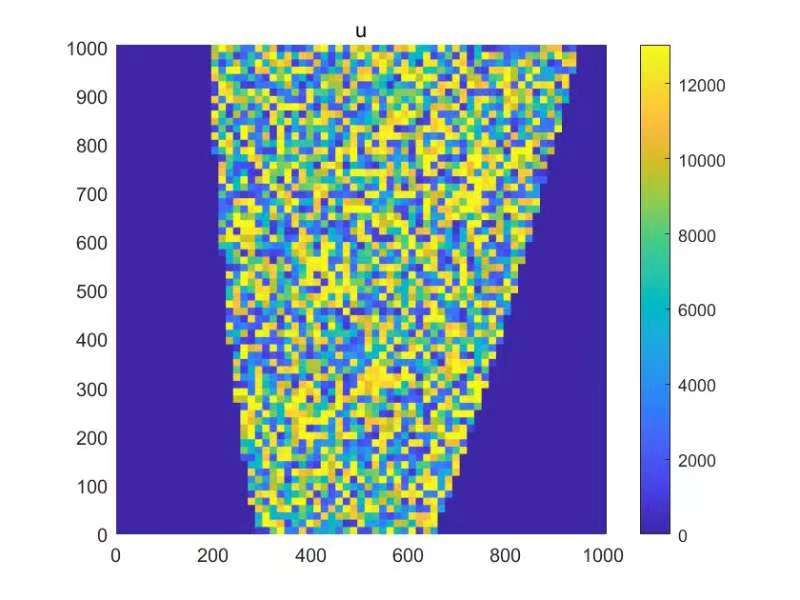
\includegraphics[width=7cm]{out7.jpeg}
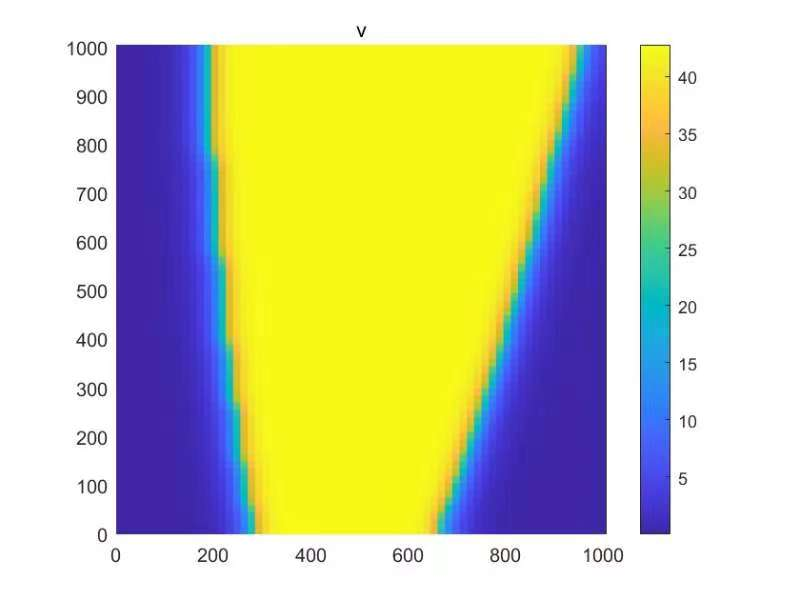
\includegraphics[width=7cm]{out8.jpeg}
\caption{$n_1 = 10000$, side length = 1000, space step = 15, time step = 1/24, maximum time = 500, Dy/Dx = 100, $u^* = 108.488, v^* = 41.844$, $U_{i,j}^0 = u^*-2\times10^{-7}(x_i-0.1y_j-225)(x_i-0.1y_j-675), V_{i,j}^0 = v^*-3\times10^{-5}(x_i-450)-1.2\times10^{-4}(y_i-150)$}
\end{figure}

\noindent For the second situation, we take $n_2$=0.000001, then the same unfortunate thing happened again. Under this situation, if we take the value of $n_1$ too large, then there will be no pattern. Therefore, the value of $n_1$ has been controlled in a range with small number.
\vspace{12pt}

\noindent If we take $n_1$=0.1,

\begin{figure}[H]
\centering
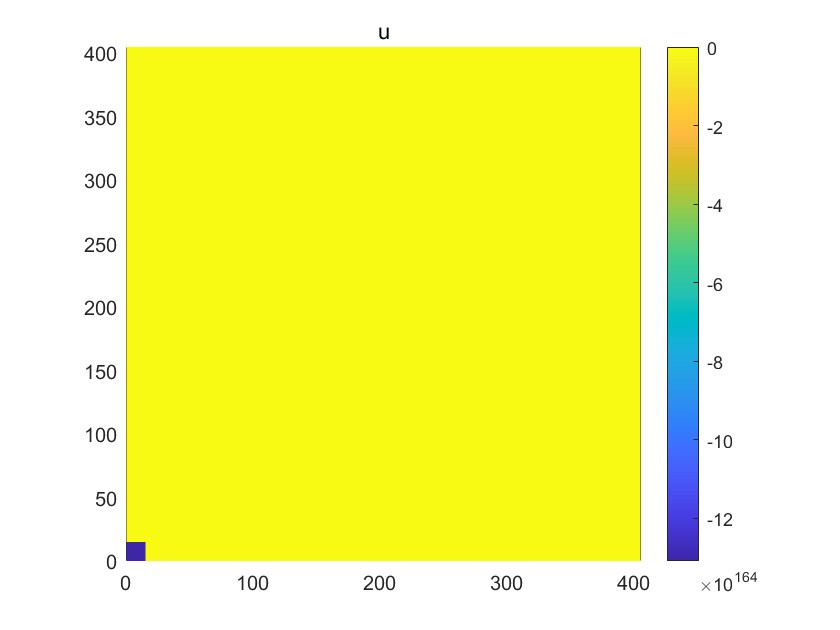
\includegraphics[width=7cm]{out9.jpeg}
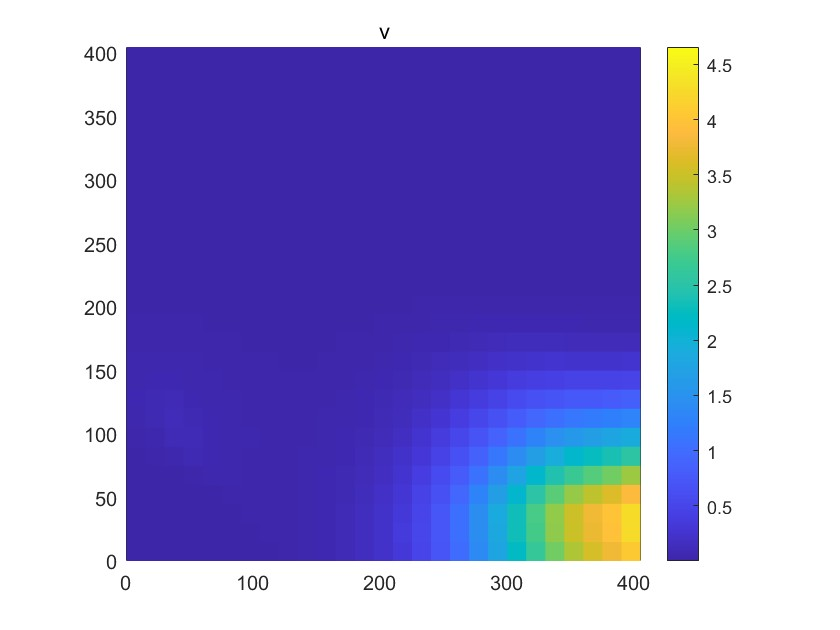
\includegraphics[width=7cm]{out10.jpeg}
\caption{$n_1 = 0.1$, side length = 400, space step = 15, time step = 1/24, maximum time = 120, Dy/Dx = 100, $u^* = 0.467, v^* = 0.00045$, $U_{i,j}^0 = u^*-2\times10^{-7}(x_i-0.1y_j-225)(x_i-0.1y_j-675), V_{i,j}^0 = v^*-3\times10^{-5}(x_i-450)-1.2\times10^{-4}(y_i-150)$}
\end{figure}

\noindent If we take $n_1$=0.01,

\begin{figure}[H]
\centering
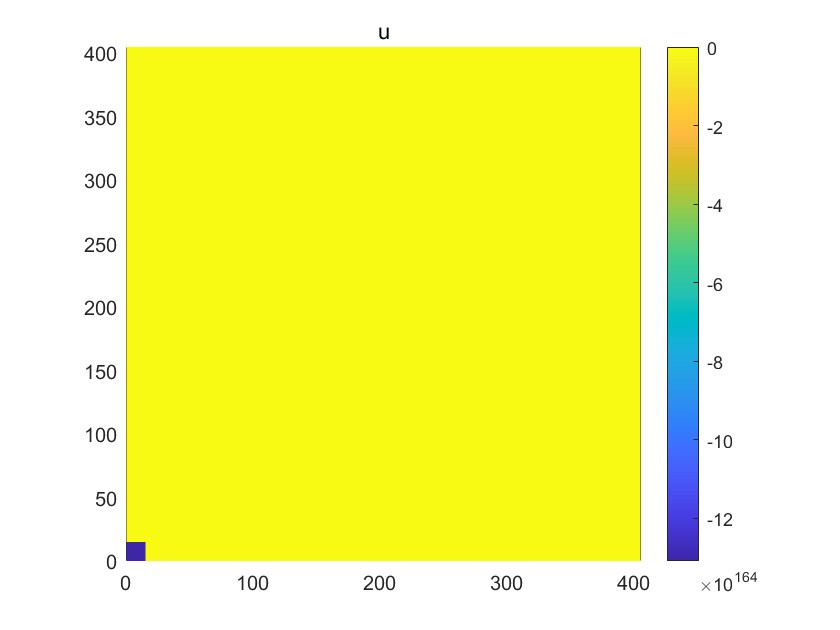
\includegraphics[width=7cm]{out11.jpeg}
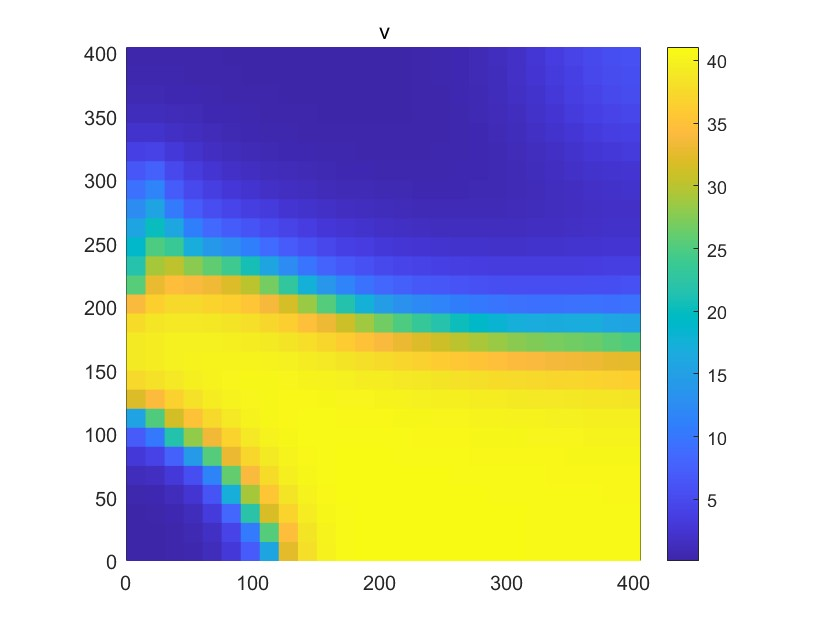
\includegraphics[width=7cm]{out12.jpeg}
\caption{$n_1 = 0.01$, side length = 400, space step = 15, time step = 1/24, maximum time = 120, Dy/Dx = 100, $u^* = 0.467, v^* = 0.00056$, $U_{i,j}^0 = u^*-2\times10^{-7}(x_i-0.1y_j-225)(x_i-0.1y_j-675), V_{i,j}^0 = v^*-3\times10^{-5}(x_i-450)-1.2\times10^{-4}(y_i-150)$}
\end{figure}

\noindent If we take $n_1$=0.001,

\begin{figure}[H]
\centering
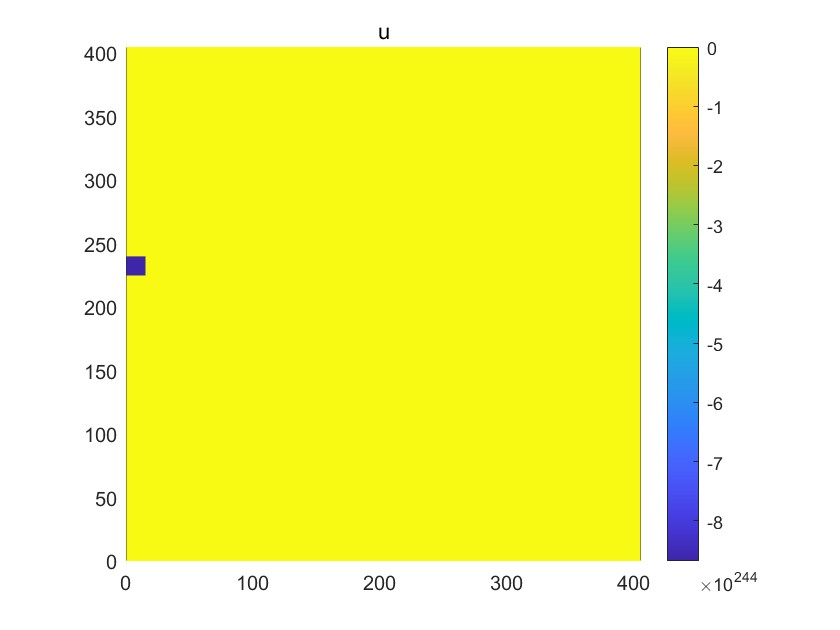
\includegraphics[width=7cm]{out13.jpeg}
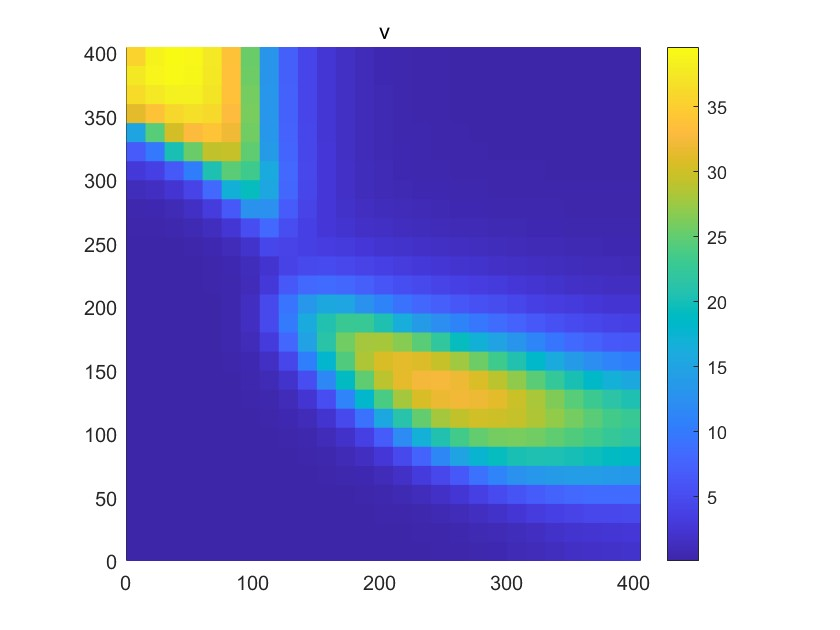
\includegraphics[width=7cm]{out14.jpeg}
\caption{$n_1 = 0.001$, side length = 400, space step = 15, time step = 1/24, maximum time = 120, Dy/Dx = 100, $u^* = 0.467, v^* = 0.00057$, $U_{i,j}^0 = u^*-2\times10^{-7}(x_i-0.1y_j-225)(x_i-0.1y_j-675), V_{i,j}^0 = v^*-3\times10^{-5}(x_i-450)-1.2\times10^{-4}(y_i-150)$}
\end{figure}

\noindent From the graph above, it can be seen that the patterns of prey almost did not change, but there was a clear change between different patterns of predator. In other words, in extreme cases, the changes in predators are more pronounced than prey’s.

\vspace{24pt}


\section{Conclusion}
\subsection{Conclusion}
\noindent In this report, we mainly introduced the given model and some corresponding-background knowledge, we derived the analytical conditions of the Turing patterns of the model, we also constructed analytical model and use MATLAB to check whether the model is capable to produce Turing patterns with different value of Allee constant. We carried out mathematical analysis to observe the qualitative and quantitative dynamics of the model when the patterns shown. We did the numerical simulations with field-based parameter values from the existing literature, please check the reference list. 
\vspace{24pt}

\noindent In the end, we find that, the Allee Effect has a significant impact on the generation of Turing patterns. The impact mainly caused by the value of Allee constant, the constant’s value will determine the range of generating the patterns and whether the Turing instability can be satisfied. However, the impact is totally different for the two variables. For example, in this paper, we checked that if we take the value of a part of Allee constant quite small, but change the other part of Allee constant, there will be a significant difference between the patterns of two variables. 
\vspace{24pt}

\noindent From Figure 7 to 9, we took the value of $n_1$ as 0.1, 0.2, and 0.3 with the value of $n_2$ was 10. The difference between each test’s value of $n_1$ was not big, but there were some clear changes between each of them, especially for the predators. We can clearly see that, the predators’ living area significantly moved upward when we made $n_1$ larger than last time. When $n_1=0.3$, all of the predators almost lived in the right-top corner while the preys prefer living in the left-down corner. There was a gradient boundary between them. As for the Figure 10 to 11, we kept the value of $n_2$ as 10 but change $n_1$ into very small. The results were impressive but if we keep making the value of $n_1$ small, the patterns will not change too much. After considering the situation with a normal value of $n_2$, we turned to consider two extreme situations: one is taking $n_2$ very large, the other is taking it very small. For the first situation, we took the value of $n_2$ as 1000. We found that there was no pattern if the value of $n_1$ was too small, therefore we tried to seek some solution with big value. We took $n_1$ as 1000 and 10000, from Figure 12 to 13 we can see that, with different equilibrium points, the preys and predators could live evenly dispersed or differentiate significantly. From Figure 14, square patterns occur which indicates that their spatial distribution is quite chaotic. From Figure 15, there were V-shaped patterns. This indicates that their spatial distribution exhibits significant differentiation overall, but also exhibits chaotic distribution locally. After that, we took the value of $n_2$ as 0.000001, similarly we found that there was no pattern if $n_1$ was too large. Hence, we took the value of $n_1$ as 0.1, 0.01 and 0.001 respectively. From Figure 16 to 18, we can find that the preys’ situation is not optimistic, we inferred that it got extincted at time T, while the predators’ spatial distribution changed a lot every time we changed the value of $n_1$. It was very interesting and mysterious, but we do not keep our study to figure out why.

\subsection{Improvement and Further work}
\noindent Although we try to explain everything in detailed logically in this paper, there was still improvement that can be done.
\vspace{24pt}

\noindent First, the model built in this paper was not perfect, recall that we wrote the Allee Effect in this form:$1-\frac{n_1+n_2}{x+n_2}$. This can only partially indicate the inhibitory effect of the Allee Effect on the growth of two organisms, especially when the value of $n_2$ had been determined already. If we want to research the Allee Effect deeply, there were two choices: the first one is this paper; the second one is to change the value of $n_i$ respectively but not to determine any of them as a constant.

\vspace{24pt}

\noindent Secondly, if we want more Turing patterns to show, then we need to try more different parameters’ value, for example, the area of the graph, the maximum time etc. can be changed. This is a task that requires a precise computer and a lot of time, there might be thousands of times to try different parameters to make some new discoveries. However, based on our experience, all the values of the mentioned parameters should be taken in a determined range but not randomly, the result will not converge to generate a graph if the value was taken out of the range.

\vspace{24pt}

\noindent Thirdly, this paper just focus on the basic Turing patterns, but there are more different conditions of Turing instability, there will be totally different result under different situation. For example, the bifurcation is a very important part of this research. The following bifurcations can be researched in this model: Turing-Hopf, Turing-Bogdanov, Turing-Transcritical, Turing-Saddle-node and Turing-Pitchfork bifurcation.

\newpage
\begin{thebibliography}{10}
\addcontentsline{toc}{section}{Reference}

\bibitem{latexGuide}Abrams, P.A., 1994. The fallacies of "ratio-dependent"predation. Ecology 75, 1842–1950.


\bibitem{latexGuide}Arditi, R., Ginzburg, L.R., 1989. Coupling in predator–prey dynamics: ratio-depen-dence. J. Theor. Biol. 139, 311–326

\bibitem{latexGuide}Arditi, R., Ginzburg, L.R., 2012. How Species Interact: Altering the Standard View on Trophic Ecology. Oxford University Press, New York.



\bibitem{latecGuide}Boukal, D.S., Berec, L., 2002. Single-species models and the Allee effect: extinction boundaries, sex ratios and mate encounters. J. Theor. Biol. 218, 375–394.

\bibitem{latecGuide}Clark, C.W., 1990. Mathematical Bioeconomic: The Optimal Management of Re-newable Resources, 2nd ed. John Wiley and Sons, New York.


\bibitem{latexGuide}Haque, M., 2009. Ratio-dependent predator–prey models of interacting populations. Bull. Math. Biol. 71, 430–452

\bibitem{latexGuide}Haque, M., 2012. Existence of complex patterns in the beddington-deangelis predator-prey model. Mathematical Bioscience

\bibitem{latexGuide}Hongju, Y., 2018. Research on Bifurcation and Pattern Self-organization of a Discrete Reaction-diffusion Predator-prey System

\bibitem{latexGuide}James, D.M., 1993. Mathematical Biology. https://link.springer.com/book/10.1007/978-3-662-08542-4

\bibitem{latexGuide}Lev, R., Ginzburg, H., Akcakaya, R., 1992. Consequences of ratio-dependent predation for steady-state properties of ecosystems. Ecology 73, 1536 1543.

\bibitem{latecGuide}Liermann, M., Hilborn, R., 2001. Depensation: evidence, models and implications. Fish Fish. 2, 33–58.

\bibitem{latecGuide}Malay, B., Vitaly, V., 2017. Spatio-temporal pattern formation in Rosenzweig–MacArthur model: Effect of nonlocal interactions, p2-10


\bibitem{latecGuide}Medvinsky,A.B., Petrovskii,S.V., Tikhonova,I.A., Malchow,H., Li,B.L., Spatiotemporal complexity of plankton and fish dynamics, Siam Review (2002) 311.

\bibitem{latecGuide}Murray, J.D., 2011. Mathematical biology: I. an introduction. Springer New York, p79-118

\bibitem{latexGuide}Nayana, M., Malay, B., 2022. Hunting cooperation among slowly diffusing specialist predators can induce stationary Turing patterns


\bibitem{latexGuide}Stephens, P. A., W. J. Sutherland, and R. P. Freckleton. “What Is the Allee Effect?” Oikos 87, no. 1 (1999): 185–90. https://doi.org/10.2307/3547011.

\bibitem{latexGuide}Turing,A.M. , The chemical basis of morphogenesis, Philosophical Transactions of the Royal Society of London Series B 237 (1952) 37.

\bibitem{latecGuide}Wang, J., Shi, J., Wei, J., 2011. Predator–prey system with strong Allee effect in prey. J. Math. Biol. 62, 291–331.


\end{thebibliography}

\newpage



\appendix

\section{Appendix}

\subsection{ Code of MATLAB}
\noindent\rule[0.25\baselineskip]{\textwidth}{1pt}
n1 = input('Enter parameter n1 ');\\
n2 = input('Enter parameter n2 ');\\
syms x y;\\
$eq1=0.8*x*(1-x/100)*(1-(n1+n2)/(x+n2))-24*x*y/(15*x+30)==0;$\\
$eq2=7.92*x*y/(15*x+30)-0.1*y-0.01*y^2==0;$\\
$[x,y]=vpasolve([eq1,eq2],[x,y])$\\
\noindent\rule[0.25\baselineskip]{\textwidth}{1pt}
x = input('Enter parameter x ');\\
y = input('Enter parameter y ');\\
$D_x = input('Enter parameter D_x ');$\\
$D_y = input('Enter parameter D_y ');$\\
n1 = input('Enter parameter n1 ');\\
n2 = input('Enter parameter n2 ');\\
syms E1 E2\\
$eq1=E1-(D_y*(0.8*(1-x/50)*(1-(n1+n2)/(x+n2))+0.8*x*(1-x/100)*(1+(n1+n2)/(x+ n2)^2-(24*y*(15*x+30)-360*x*y)/(15*x-30)^2))+D_x*(7.92*x/(15*x-30)-0.1-0.02 *y))==0;$\\
$eq2=E2-(((0.8-16*x/1000)*(1-(n1+n2)/(x+n2))+0.8*x*(1-x/100)*(1+(n1+n2)/(x+n 2)^2)-225*y/(10*x+15)^2)*(7.92*x/(15*x+30)-0.1-0.02*y)-(-24*x/(15*x+30)*(23 7.6*y/(15*x+30)^2)))==0;$\\
$[E1,E2]=vpasolve([eq1,eq2],[E1,E2])$\\
\noindent\rule[0.25\baselineskip]{\textwidth}{1pt}
E1 = input('Enter parameter E1 ');\\
E2 = input('Enter parameter E2 ');\\
$D_x = input('Enter parameter D_x ');$\\
$D_y = input('Enter parameter D_y ');$\\
syms I1 I2 I3\\
$eq3=I1-E1==0;$\\
$eq4=I2-(E1-2*(D_x*D_y*E2)^0.5)==0;$\\
$eq5=I3-E2/(D_x*D_y)==0;$\\
$[I1,I2,I3]=vpasolve([eq3,eq4,eq5],[I1,I2,I3])$\\
\noindent\rule[0.25\baselineskip]{\textwidth}{1pt}
n1 = input('Enter parameter n1 ');\\
n2 = input('Enter parameter n2 ');\\
$a = input('Enter a in [a,b]^2 ');$\\
$b = input('Enter b in [a,b]^2 ');$\\
h = input('Enter space-step h ');\\
T = input('Enter maximum time T ');\\
delt = input('Enter time-step Delta t ');\\
delta = input('Enter parameter delta ');\\
U0 = input('Enter initial data function U0(X,Y) ','s');\\
V0 = input('Enter initial data function V0(X,Y) ','s');\\
% User inputs of initial data
$mu=delt/(h^2);$\\
J=round((b-a)/h);\\
dimJ=J+1;\\
$n = (dimJ)^2;$\\
\% no. of nodes (d.f.) for each dependent variable N=round(T/delt);\\
\% Initialization\\
$u=zeros(n,1); v=zeros(n,1); F=zeros(n,1);$\\
$G=zeros(n,1); y1=zeros(n,1); y2=zeros(n,1); $\\
$U_grid=zeros(dimJ,dimJ);$\\
$ V_grid=zeros(dimJ,dimJ); B=sparse(n,n); L=sparse(n,n);$\\
\% Assign initial data\\
indexI=1:dimJ;\\
x=(indexI-1)*h+a;\\
$[X,Y]=meshgrid(x,x);$\\
$U0 = eval(U0).*ones(dimJ,dimJ); V0 = eval(V0).*ones(dimJ,dimJ);$\\
\% Change orientation of initial data & convert to 1-D vector \\
U0=U0'; V0=V0'; u=U0(:); v=V0(:);\\
$\% Construct matrix L (without 1/h^2 factor)$\\
L(1,1)=3; L(1,2)=-3/2; L(J+1,J+1)=6; L(J+1,J)=-3;\\
L=L+sparse(2:J,3:J+1,-1,n,n);\\
L=L+sparse(2:J,2:J,4,n,n);\\
L=L+sparse(2:J,1:J-1,-1,n,n);\\
L(1,J+2)=-3/2; L(J+1,2*J+2)=-3; \\
L=L+sparse(2:J,J+3:2*J+1,-2,n,n);\\
L(n-J,n-J)=6; L(n-J,n-J+1)=-3;\\
L(n,n)=3; L(n,n-1)=-3/2;\\
L=L+sparse(n-J+1:n-1,n-J+2:n,-1,n,n); \\
L=L+sparse(n-J+1:n-1,n-J+1:n-1,4,n,n); \\
L=L+sparse(n-J+1:n-1,n-J:n-2,-1,n,n);\\
L(n-J,n-(2*J+1))=-3; L(n,n-dimJ)=-3/2; \\
L=L+sparse(n-J+1:n-1,n-2*J:n-(J+2),-2,n,n); \\
L=L+sparse(J+2:n-dimJ,2*J+3:n,-1,n,n); \\
L=L+sparse(J+2:n-dimJ,1:n-2*dimJ,-1,n,n); \\
L=L+sparse(J+2:n-dimJ,J+2:n-dimJ,4,n,n); \\
L=L+sparse(J+2:n-(J+2),J+3:n-dimJ,-1,n,n); \\
L=L+sparse(J+2:dimJ:n-(2*J+1),J+3:dimJ:n-2*J,-1,n,n); \\
L=L+sparse(2*J+2:dimJ:n-2*dimJ,2*J+3:dimJ:n-(2*J+1),1,n,n); \\
L=L+sparse(J+3:n-dimJ,J+2:n-(J+2),-1,n,n); \\
L=L+sparse(2*J+2:dimJ:n-dimJ,2*J+1:dimJ:n-(J+2),-1,n,n); \\
L=L+sparse(2*J+3:dimJ:n-(2*J+1),2*J+2:dimJ:n-2*dimJ,1,n,n);\\
\% Construct matrices B1 & B2\\
B1=sparse(1:n,1:n,1,n,n)+mu*L; \\
B2=sparse(1:n,1:n,1,n,n)+delta*mu*L;\\
\% Time-stepping procedure\\
for nt=1:N\\
\% Evaluate modified functional response\\
hhat = u./(15.*abs(u) +30);\\
\% Update right-hand-side of linear system\\
F = (0.8).*u.*(1-u./100).*(1-(n1+n2)./(u+n2))-24.*v.*hhat\\
$G = (7.92.*v).*hhat-(0.1).*v-(0.01).*v.^2;$\\
y1 = u + delt*F;\\
y2 = v + delt*G;\\
\% Solve for u and v using GMRES\\
[u,flagu,relresu,iteru]=gmres(B1,y1,[],1e-6,[],[],[],u);\\
if flagu~=0 flagu,relresu,iteru,error('GMRES did not converge'),end\\
[v,flagv,relresv,iterv]=gmres(B2,y2,[],1e-6,[],[],[],v);\\
if flagv~=0 flagv,relresv,iterv,error('GMRES did not converge'),end\\
end\\
\% Re-order 1-D solution vectors into 2-D solution grids\\
$V_grid=reshape(v,dimJ,dimJ); U_grid=reshape(u,dimJ,dimJ);$\\
\% Put solution grids into ij (matrix) orientation\\
$V_grid=V_grid'; U_grid=U_grid';$\\
\% Plot solutions u and v\\
$figure;pcolor(X,Y,U_grid);shading flat;colorbar;axis square xy;title('u')$\\
$figure;pcolor(X,Y,V_grid);shading flat;colorbar;axis square xy;title('v')$\\



\end{document}